\documentclass[master, tikz, final,11pt, dvipdfmx]{iscs-thesis}

\usepackage{amsmath}
\usepackage{amsfonts}
\usepackage{caption}
\usepackage{lipsum}
\usepackage{subcaption}
\usepackage{graphicx}
\graphicspath{ {./figures/} }
\usepackage[table]{xcolor}
\newcommand{\norm}[1]{\left\lVert#1\right\rVert}
\usepackage[utf8]{inputenc}
%\usepackage{url}
\usepackage{hyperref}
\hypersetup{
    colorlinks,
    citecolor=black,
    filecolor=black,
    linkcolor=black,
    urlcolor=black
}
\hypersetup{linktocpage}
\usepackage{multirow}
\usepackage{tikz}
\usetikzlibrary{matrix,chains,intersections,positioning,decorations.pathreplacing,arrows,shapes, arrows, calc}

%\usepackage[T1]{fontenc}

%-------------------
\etitle{Adaptive Neural Networks Layer for Multi-Speaker Separation Problem}
\jtitle{Multi-Speaker問題に対するAdaptive Networks Layerについての研究}
%
\eauthor{Anthony D'Amato}
\jauthor{アントニー ダマト}
\esupervisor{Hiroshi Imai}
\jsupervisor{今井 浩}
\supervisortitle{Professor} % Professor, etc.
\date{January 29, 2018}
%-------------------
\begin{document}


\begin{eabstract}

The complexity of sound, its noisy character and the overlapped information makes the single channel Multi-Speaker Separation quite a challenge for the audio signal processing area. In comparison, humans are very good at distinguishing different voices in complex environments.

One of the first successful approach for this problem was to use non-negative matrix factorization (NMF), sparse NMF and later convolutional NMF but these methods had some drawbacks because of their linearity, cost and weak representation.

With the arrival of Deep Learning in audio signal processing, improvements have been made in denoising, audio classification, and mostly in Natural Language Processing  (NLP) with the recent WaveNet and Tacotron 2 architectures. In the recent years new techniques involving Deep Learning were proposed and are performing quite well in the Multi-Speaker Separation problem. These latter are based on producing masks for mixed spectrograms to separate voices. To do so, they apply bidirectional recurrent neural networks on spectrograms trained to produce embeddings representing each speaker. This created embedded space allows to apply unsupervised algorithms such as k-means to segment the spectrograms and create binary masks. Contrary to the previous class-based segmentation methods, these new approaches are partition-based segmentation and lead to a speaker-independent inference and therefore easier generalization and precision. These approaches could reach more than 11dB improvement for the Signal to Distortion Ratio (SDR) in average for separating male and female mixed voices.

But these methods still struggle to separate mixed voices of the same gender and thus struggle to separate more than three voices from a single input channel. We presume that this problem might be mainly due to the overlapping frequencies in the mixed spectrograms when the same genders are speaking. To overcome this issue, we replace the use of spectrograms and propose a new approach consisting in using a sparse linear autoencoder, named 'adaptive layer', added to the current state of the art methods, namely the Deep Clustering (DPCL) and Source Contrastive Estimation (SCE) approaches. This autoencoder is composed of two main parts, a front-end layer and a back-end layer, and is able to take in input raw mixed audio signals and output separated audio signals. 

In this study, we compare the SDR improvements with and without the adaptive layer for a mixture of different speakers. Furthermore, we improve the SCE approach using methods introduced by Deep Clustering and other new regularization methods, we show that we can increase the SDR improvement of SCE method by 1.14dB.

\end{eabstract}

\maketitle

\begin{acknowledge}

Firstly, I would like to express my gratitude to my supervisor Hiroshi Imai for his support and wise advice all along this thesis, in addition, I would like to deeply thank Hidefumi Hiraishi and Naoto Ohsaka who helped me a lot over these years. I would also like to thank Doctor Yoshizoe of RIKEN AIP for all his feedback and support, and for accepting me in his unit as a trainee and allowing me to use RAIDEN computer without which I would not have been able to realize all this work.

Secondly, I would like to especially thank Natalia Jarzebska and Dea Luma for all their support throughout these 2 years and a half in Japan, having them by my side was a huge source of motivation and inspiration. Thank you for all your advice, for having listened to me, and for all the amazing moments we spent together, I will never forget everything you did for me.

Finally, I would like to express my profound gratitude to all my familly for all their support all over these years, even with the distance they continued to always be by my side and encouraging me to do my best.

\end{acknowledge}

\pagenumbering{arabic}

\newpage

\tableofcontents

\newpage

\listoffigures % Prints the list of figures

\listoftables % Prints the list of tables


\chapter{Introduction}

%\nocite{*}

\section{Multi-Speaker Separation Problem}
In 1953, Colin Cheery called the capacity of human beings to separate many voices in a conversation the \textit{cocktail party problem}. We know that humans are very good at separating voices or other sounds from a noisy environment by focusing their attention to a particular chosen target. In this study, we focus our attention on the multi speaker separation problem consisting in separating from a \textbf{single channel} a mixture of speakers with different genders. 

More generally, the source separation problem can be very useful in domains like automatic speech recognition, speech enhancement for hearing aids or in music tracks separation.

One challenge in the source separation problem is called the '\textit{permutation problem',} that is happening when segmentation is used to separate the sources without having knowledge of the separated sources, therefore we do not know which partition belong to which source. This is a problem when chunking the input in order to process it in a separating model, the first chunk will output a certain order for the separation but it is not assured that next chunks will be outputted in the same order. We will discuss later in this study about how new deep learning architectures are solving this problem.

In this study, we only focus on the \textbf{single channel separation problem} but multi-channel audio separation is as well a very active area that has shown to produce even better results than using a unique channel. Today's deep learning methods, such as Deep Clustering \cite{DPCLV1, DPCLV2} can achieve quite good results in the multi speaker separation problem for 2 different genders speakers mixtures in terms of SDR improvements but are still not obtaining as successful results for \textbf{speakers of the same gender} or for a mixture of more than 2 speakers. 

The main advantage brought by Deep Clustering \cite{DPCLV1} method is that it is a partition-based segmentation where the labels of the partitions are learned in opposition of a class-based segmentation where the labels of the segmented sources are learned. This approach allows to generalize very well to unknown speakers because it does not learn '\textit{who}' is speaking but how to differentiate each speaker without the '\textit{who}' information. Deep Clustering method produces discriminative embeddings from spectrogram magnitudes to apply clustering algorithm on them and then assign labels to each partitions. These learned partitions are used to create masks for the input spectrograms and separate each voice.

In this study we intend to improve the performances of current state of the art methods regarding same gender mixtures.

Firstly, this study is in part based on \cite{Adaptive} which shows that using an end-to-end autoencoder architecture on raw audio mixture for the source separation problem instead of Discrete Cosine Transform spectrograms can lead to better SDR improvement but this study is limited in terms of number of separated speakers, deep neural network complexity and generalization error. We suppose that a similar architecture, compatible with current state of the art deep learning methods and replacing the use of spectrograms, can lead to better results. In addition, we suppose that one problem with the use of spectrograms is that for a mixture of speakers with the same gender it is more likely that frequencies overlapping occurs, and thus separating information becomes more challenging. The architecture we propose to replace the use of spectrogramw tries to decrease this overlapping problem and thus intends to increase performances with mixtures of the same gender. 

Secondly, we consider another approach named Source Contrastive Estimation (SCE) \cite{SCE} that is based on the same principles than Deep Clustering and has shown to have better results. Indeed, since SCE method delivers better SDR improvement than the first version of Deep Clustering \cite{DPCLV1} and since the methods used in its second version \cite{DPCLV2} can be applied to any other methods, we presume that applying such improvements to SCE can lead to an enhancement of its performances.


\section{Contributions}
\label{contrib}

In our work we are adressing the improvement of the multi speaker separation problem with two main approaches:

Firstly, we propose a sparse autoencoder architecture to replace the use of spectrogram and lower the overlapping in the usual representation. We show that this neural network can improve the performances for 2 speakers mixtures but creating such an architecture for a mixture of 3 speakers is more challenging.

Secondly and in parallel, we improve the Source Contrastive Estimation method using different techniques brought by the second version of Deep Clustering \cite{DPCLV2}. In addition, we try new regularization techniques for SCE such as Negative Sampling or combining it with the DANet \cite{DANet} method. We show that all these combinations can lead to significant improvements of the SCE method.

\chapter{Background}
\section{The Short Time Fourier Transform (STFT)}

\begin{figure}[h]
\centering
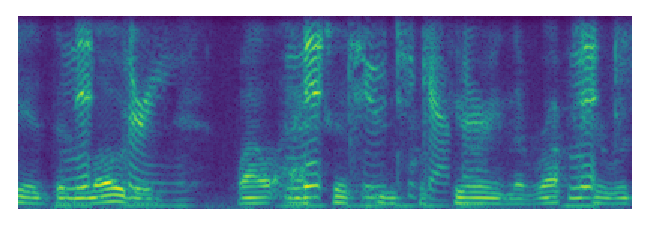
\includegraphics[width=0.8\textwidth]{xmix}
\caption[Spectrogram of a 2 speaker mixture]{Spectrogram of a 2 speakers mixture using the square root of the Hann function as window of size 256 and a hop size of 64. The length of the audio signal used is of 26368 frames ($\simeq 3.3$ seconds),and in this case $F = 129$ and $T = 409$.}
\label{fig:spectrogram} 
\end{figure}


Short-Time Fourier Transform (STFT) has played a significant role in signal processing research and has been broadly used in many applications involving sounds analysis.
This transformation on a signal is obtained by applying the Fourier Transform along it on a fixed-sized window and moving it along with some overlapping. This operation converts this signal that has frequency changes over time into a time-frequency domain that can be more understable for analysis than its original 1-dimensional representation.
The STFT of a signal $x$ at the frame $t$ and frequency $f$, named the \textit{TF-bin}, is defined as follow:
\[
	STFT\{x\}(t,f) = X(t,f) = \sum_{n=-\infty}^{n=+\infty}x[n]w[t-mh]e^{-jf\frac{2\pi}{N}t } \in \mathbb{C}^{T\times F}
\]

Here, $f$ designates the frequency index, $t$ is the frame center and $h$ the hop size. The \textit{analysis window} used for the tranformation is $w$ and is of size $N$. The most commonly used analysis windows are the Hann and Hamming windows.
The STFT of a signal $x$ can be seen as a complex matrix $X \in \mathbb{C}^{T\times F}$ ($T$ representing the time axis and and $F$ the frequency axis) that can be decomposed as follow:

\[
	STFT\{x\} = X = |X|\exp^{j\phi}
\]

In this decomposition, $|X|$ represents the STFT magnitude and $\phi$ its phase. In audio analysis, what is called the \textit{\textbf{spectrogram}} (\autoref{fig:spectrogram}) of an audio signal is the squared magnitude of the computed Short-Time Fourier Transform and is defined as follow:

\[
	spectrogram\{x\}(t,f) =  |X(t,f)|^2
\]

In this study, we consider a mixture of $M$ speakers ,with the same or of a different gender, $x$ defined as:

\[
x = \sum_{i=0}^{M} x_i
\]

Here, $x$ is named the \textit{\textbf{mixture}} and each $x_i$ are the \textit{\textbf{original sources}}. Since the STFT is a linear operation, applying it on the mixture leads to:

\[
	STFT\{x\} = X = \sum_{i=0}^{M} X_i =\sum_{i=0}^{M} STFT\{x_i\}
\]

Since complex numbers are difficult to handle in audio processing, the phase is most of the time discarded and only the magnitude is used. Even if some information might be lost by discarding the phase, studies \cite{stft} have shown that for small window size (20 - 40ms) most of the information is contained in the STFT magnitude. It has been as well shown that, even if the absolute value is taken into account, the additivity approximately holds regarding and thus that: $|X| \simeq \sum_{i=0}^{M} |X_i|$. This property and the non-negativity of spectrograms lead to the use of masks in order to perform source separation.


\section{Spectrogram Masking}

Masking is a technique broadly used for speech denoising or source separation. It consists in applying element-wisely a matrix $m^{T \times F \times M}$ to separate $M$ sources from the mixture or $m \in R^{T \times F}$ for the speech enhancement case since it is only desired to separate noise from one specific source. Since the STFT representation for audio signals is sparse, it is likely that a specific source is dominant at a particular bin in terms of energy. This property and the non-negativity of the STFT magnitude motivated the use of masks in order to separate sources from an unique spectrogram.

The \textit{\textbf{ideal binary mask}} $IBM(t,f)_i$ applied at a $(t,f)$ bin for the $i^{th}$ speaker is defined as:
\[
m^{ibm}_i(t,f) = IBM(t,f)_i = \left\{
    \begin{array}{ll}
        1 & \mbox{if } |X(t,f)_i| > max_{j \neq i} |X(t,f)_j \\
        0 & \mbox{else}
    \end{array}
\right.
\]

The ideal binary mask can be seen as a matrix $m^{ibm} \in R^{T\times F \times M}$ where an element at $(t,f,i)$ is set to $1$ for the $i^{th}$ speaker if this latter is dominant compared to the others and $0$ otherwise. In \cite{IBM}, it is shown that IBM can be very efficient for separating sources but highly depends on the STFT window size, and this optimal can vary according to the source type and task.

Another popular mask is the \textit{\textbf{Wiener-like filter}}, which generally leads to better Signal to Distortion Ratio (SDR) since it is a softer masks of which values lands in [0,1]. The Wiener-like filter is defined as:
\[
m^{wf}_i = \frac{|X_i|^2}{\sum_j{|X_j|^2}} 
\]

We show the difference between binary and Wiener-like masks in \autoref{fig:masking}.
In the result section \ref{res} we compare our results with the Wiener-like filters.


\begin{figure}[h]
\centering
\begin{subfigure}[b]{0.9\textwidth}
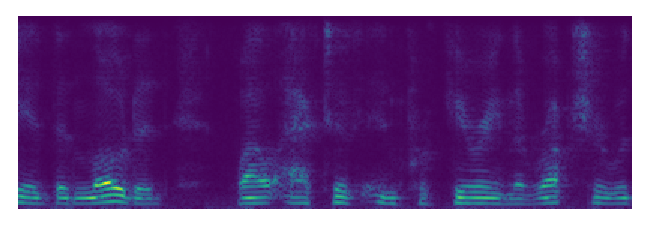
\includegraphics[width=\textwidth]{xnonmix1}
\caption{Spectrogram of the $1^{st}$ speaker from \ref{fig:spectrogram}}
\label{fig:nonmix1} 
\end{subfigure}
\\
\begin{subfigure}[b]{0.45\textwidth}
\includegraphics[width=\textwidth]{ibm1}
\captionsetup{justification=centering}
\caption{Binary mask extracting the  $1^{st}$ speaker}
\label{fig:ibm1} 
\end{subfigure}
~
\begin{subfigure}[b]{0.45\textwidth}
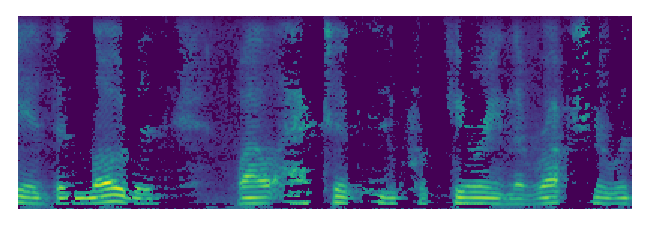
\includegraphics[width=\textwidth]{sepibm1}
\captionsetup{justification=centering}
\caption{Reconstruction using the binary mask}
\label{fig:ibmsep1} 
\end{subfigure}
\\
\begin{subfigure}[b]{0.45\textwidth}
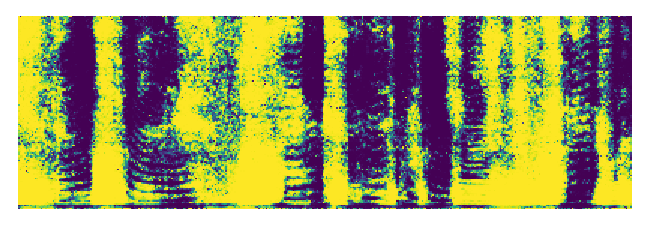
\includegraphics[width=\textwidth]{wf1}
\captionsetup{justification=centering}
\caption{Wiener-like mask extracting the  $1^{st}$ speaker}
\label{fig:wf1} 
\end{subfigure}
~
\begin{subfigure}[b]{0.45\textwidth}
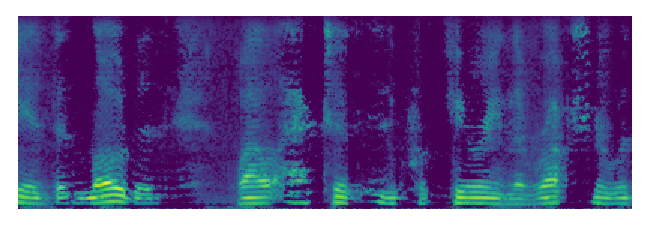
\includegraphics[width=\textwidth]{sepwf1}
\captionsetup{justification=centering}
\caption{Reconstruction using the Wiener-like mask}
\label{fig:ibmsep1} 
\end{subfigure}
\captionsetup{justification=centering}
\caption[IBM and Wiener-like masks comparison]{Comparison between binary masks and Wiener-like masks. As mentioned, we can see that using Wiener-like (\autoref{fig:wf1}) that are softer than binary masks (\autoref{fig:ibm1}) is leading to a better reconstruction}
\label{fig:masking} 

\end{figure}

\section{Deep Learning}

Deep Learning \cite{DL, DLBOOK} has seen an explosion of interest these last years and is now applied in many fields in machine learning such as classification, clustering, generation or prediction. In this section we present basic deep learning concepts such as Feed Forward Networks (FFN), Convolutional Neural Networks (CNN) and Recurrent Neural Networks. Furthermore, we explain more complex structures that we encounter in this study like Bidirectional Long Short Term Memory (BLSTM) cells and sparse autoencoder.

\subsection{Feed Forward Networks}
\label{ffn}
\begin{figure}[!hb]

\centering
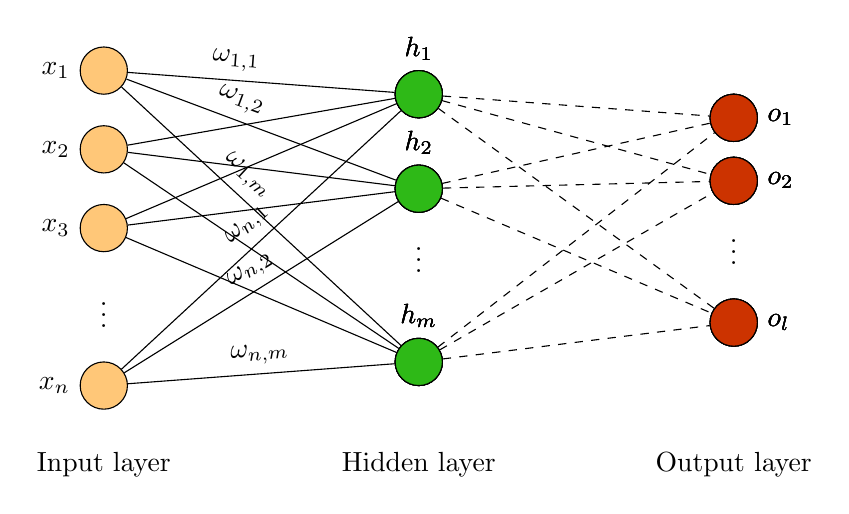
\begin{tikzpicture}

[   cnode/.style={draw=black,minimum width=10mm, circle}, ]
    \node at (0,-4) {$\vdots$};
    \node at (4,-3.3) {$\vdots$};
    \node at (8,-3.2) {$\vdots$};
    \node at (0,-6) {Input layer};
    \node at (4,-6) {Hidden layer};
    \node at (8,-6) {Output layer};
    \foreach \x in {1,...,4}
    {   
    \pgfmathparse{\x<4 ? \x : "n"}
        \node[draw=black, minimum width=6mm, circle, fill={rgb:orange,1;yellow,2;pink,5},label=180:$x_{\pgfmathresult}$] (x-\x) at (0,{-\x-div(\x,4)}) {};
        
	
	 \foreach \x in {1,...,3}
    {
    \pgfmathparse{\x<3 ? \x : "m"}
        
        \node[draw=black, minimum width=6mm, circle,fill={rgb:red,1;green,4;blue,0.5},label=90:$h_{\pgfmathresult}$] 	(p-\x) at (4,{-0.1-1.2*\x-div(\x,3)}) {};
    }
    
    \foreach \x in {1,...,3}
    {
    \pgfmathparse{\x<3 ? \x : "l"}
        
        \node[draw=black, minimum width=6mm, circle,fill={rgb:red,4;green,1;blue,0},label=0:$o_{\pgfmathresult}$] 	(o-\x) at (8,{-0.8-0.8*\x-div(\x,3)}) {};
    }
    
    
    }   
    
    
    
    \foreach \x in {1}
    {   \foreach \y in {1,...,3}
        {   
          \pgfmathparse{\y<3 ? \y : "m"}
        \draw (x-\x)-- node[above,sloped,pos=0.4] {$\omega_{\x , \pgfmathresult}$} (p-\y);
        }
    } 
    
    \foreach \x in {2,...,3}
    {   \foreach \y in {1,...,3}
        {   \draw (x-\x) -- (p-\y);
        }
    }
    
    \foreach \x in {4}
    {   \foreach \y in {1,...,3}
        {   
        \pgfmathparse{\y<3 ? \y : "m"}        
        \draw (x-\x) -- node[above,sloped,pos=0.5] {$\omega_{n , \pgfmathresult}$} (p-\y);
        }
    }
    
    \foreach \x in {1,...,3}
    {   \foreach \y in {1,...,3}
        {   \draw[dashed] (p-\x) -- (o-\y);
%            \draw[line width=2] (p-\x) to node (midf) [pos=.3, fill=white, minimum width = .8cm] {} (o-\y);
%            \draw[dot diameter = 2pt, dot spacing = .3cm, dots] (midf.east) to (midf.west);
        }
    }
    
    
\end{tikzpicture}
\caption{Example of a fully connected neural network with several hidden layers}
\label{fig:ann}
\end{figure}

Artificial Neural Networks (ANN) are based on the biological observation of human brain and how actual neurons networks are working. A human brain contains approximately 100 billions neurons that are connected to each other, studies say that an neuron has in average around 50000 connections with other neurons. They are connected to each other by what is called the \textit{synapses}.
Articial neurons are mimicking the process of biological neurons in two main steps: firstly, they take in input many other artificial neurons outputs and magnify it with a certain \textit{weight}, secondly, depending on the outcome of this operation an activation function will determine how much of this output must be outputted to other neurons it is connected to. This process is explained in \autoref{fig:ann} and can be formulated as:


\[
	h_{i}(x) = f(\sum_{j}{w_{i,j}\cdot x_j} + b_i)
\]

\[
	h(x) = f(W \cdot x + b)
\]

Here, $W$ is named the weights of the neuron layer and $b$ the biases. The function $f$ is named the activation function and decides how much information is transmitted to the next layer. This operation can be repeated several times and thus form a multi-layered feed forward network, as well named fully connected layers since all the neurons is each layer are connected to each other. \cite{FFN} has shown that this structure can approximate any functions. The intermediate layers are named the \textit{hidden} layers and the last one is logically named the \textit{output} layer.

Previously, the most commonly used activation functions were the sigmoid and the hyperbolic tangent, but because of their particular derivatives they caused either vanishing or exploding gradient. We explain this phenomenon in \autoref{loss}. 

\[sigmoid(x)  = \frac{1}{1+e^{-x}}\]
\[tanh(x)  = \frac{e^x - e^{-x}}{e^x + e^{-x}}\]

The new commonly used activation functions are the Rectified Linear Unit (ReLU), it's leaky version (leaky ReLU) and the Exponential Linear unit. All these activation functions reduce the vanishing gradient problem encountered with the previous one, and in particular ReLU functions are used for their computation efficiency.

\[ReLU(x)  = max(0,x)\]
\[ReLU_{\alpha}(x)  = max(\alpha x, x), \alpha 	\leq 1 \]
\[ELU(x)  = \left\{
    \begin{array}{ll}
        x & \mbox{if } x \geq 0 \\
        \alpha (e^x-1) & \mbox{otherwise}
    \end{array}
\right. \]

\subsection{Convolutional Neural Networks}


\begin{figure}[!h]

\includegraphics[width=\textwidth]{lenet}

	\caption[Architecture of a traditional convolutional neural network.]{LeNet-5 convolutional network architecture introduced by Y. LeCun . In this figure, we see that CNN are made of an alternation between convolutional operations (with a non linear activation function applied) and subsampling operations. This architecture was used on digits recognition}
	\label{fig:cnn}
\end{figure}


Convolutional Neural Networks (CNN or ConvNet) \cite{unpool,CNNrecent} (\autoref{fig:cnn}) are networks made from the same artificial neurons presented previously, but do not apply the same operations as fully connected networks.
The interest for CNNs increased a lot after AlexNet deep learning architecture won the ILSVRC competition in 2012 using this convolutional networks and improved previous state of the art method by almost 11\%. From then, deeper and more complex CNN networks have been built and constantly improving their accuracy.
The main difference with fully connected networks is that, as its name suggests, CNN are using convolutional operations with \textbf{\textit{filters/kernels}} along their inputs in order to create a \textbf{\textit{feature map/receptive field}}.

Image analysis began to be very difficult to use with fully connected networks because, for $256\times 256$ images for instance, the input has to be flatten and as a result the number of weights in the networks becomes very large. In CNN this problem is solved using filters that are shared across the receptive field, and thus considerably decreasing the number of weights used in the architecture.

Today's common CNN architectures, used for image analysis for instance, are made of blocks computing the following operations: first, a \textbf{convolution} operation is applied on the input with several filters on each channel of the input (for instance images can be made of red, green and blue channels), then a non-linear activation function is applied and finally a subsampling operation such as maxpooling or average pooling is applied, like it is shown in \autoref{fig:cnn}.

In our study, with the Adaptive layer (\autoref{adapt}) we use one-dimensional convolution layers along audio signal in order to learn useful filter-banks for the multi speaker separation problem.

\subsection{Recurrent Neural Networks}

Compared to vanilla feed forward networks, recurrent neural networks (RNN) are ANNs with recurrent connections, they are made of hidden states evolving in a non-linear dynamic way and
are mostly used with sequential learning.

\[
h^{t} = f(W_h \cdot h^{t-1} + W_{xh} \cdot x^t + b_h)
\]
\[
y^t = g(W_{hy} \cdot h^t + b_{hy} )
\]



\begin{figure}[h]
\centering
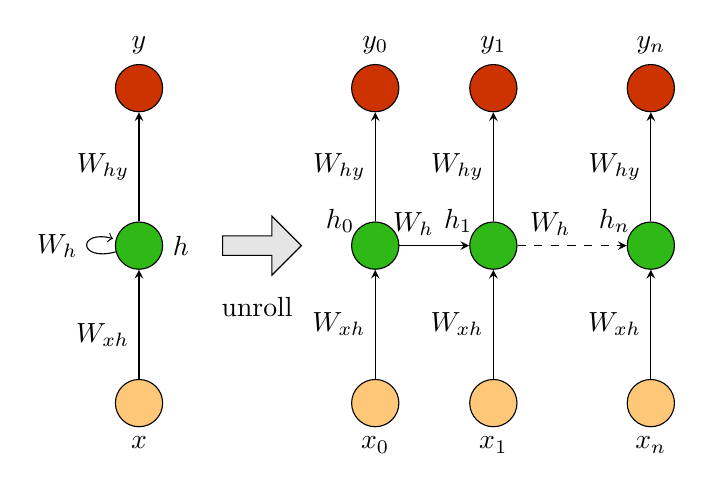
\begin{tikzpicture}

[   cnode/.style={draw=black, circle}, ]
    
    \node[draw=black, minimum width=6mm, circle, fill={rgb:red,4;green,1;blue,0},label=90:$y$] (y) at (0,2) {};
    
    \node[draw=black, minimum width=6mm, circle, fill={rgb:red,1;green,4;blue,0.5},label=0:$h$] (h) at (0,0) {};
 
    \node[draw=black, minimum width=6mm, circle, fill={rgb:orange,1;yellow,2;pink,5},label=270:$x$] (x) at (0,-2) {};
    
    \draw[->,>=stealth] (x) -- node[left,pos=0.4] {$W_{xh}$} (h);
    \draw[->,>=stealth] (h) -- node[left,pos=0.5] {$W_{hy}$} (y);
    \path (h) edge [loop left] node[left,pos=0.5] {$W_{h}$} (h);
    
    \node[single arrow,draw=black,fill=black!10,minimum height=1cm,shape border rotate=0,label={[label distance=0.4cm]270:unroll}] at (1.5,0) {};

\foreach \x in {0,...,2}
{
 \pgfmathparse{\x<2 ? \x : "n"}  \let\index\pgfmathresult
 \pgfmathparse{\x<2 ? 0 : 0.5}  \let\jump\pgfmathresult

   
    \node[draw=black, minimum width=6mm, circle, fill={rgb:red,4;green,1;blue,0},label=90:$y_\index$] (y\x) at (3+\jump +1.5*\x,2) {};
    
    \node[draw=black, minimum width=6mm, circle, fill={rgb:red,1;green,4;blue,0.5}, label={[label distance=1pt,  yshift=-0.2cm,xshift=0.1cm]135:$h_\index$}] (h\x) at (3+\jump +1.5*\x,0) {};
 
    \node[draw=black, minimum width=6mm, circle, fill={rgb:orange,1;yellow,2;pink,5},label=270:$x_\index$] (x\x) at (3+\jump+1.5*\x,-2) {};
    
    \draw[->,>=stealth] (x\x) -- node[left,pos=0.5] {$W_{xh}$} (h\x);
    \draw[->,>=stealth] (h\x) -- node[left,pos=0.5] {$W_{hy}$} (y\x);

}
    
    \draw[->,>=stealth] (h0) -- node[above,sloped,pos=0.2] {$W_h$} (h1);
    \draw[->,>=stealth, dashed] (h1) -- node[above,sloped,pos=0.3] {$W_h$} (h2);
    
\end{tikzpicture}
\caption{Example of a vanilla Recurrent Neural Network (RNN)}
\label{fig:rnn}
\end{figure}

But one of drawback of Recurrent Neural Networks is that they have problem memorizing information or context for long sequences and this is mainly due to the vanishing gradient problem \cite{RNNexploding}.


Long Short Term Memory architectures \cite{LSTM} (\autoref{fig:lstm}) are solving this problem by using a ''memory cell'' that is transiting the main information using linear operations. As its name suggests, this architecture can learn long-term dependencies.
The chained structure is kept but cells do not interact with the input the same way classical RNNs do. 

\begin{figure}[h]
\centering
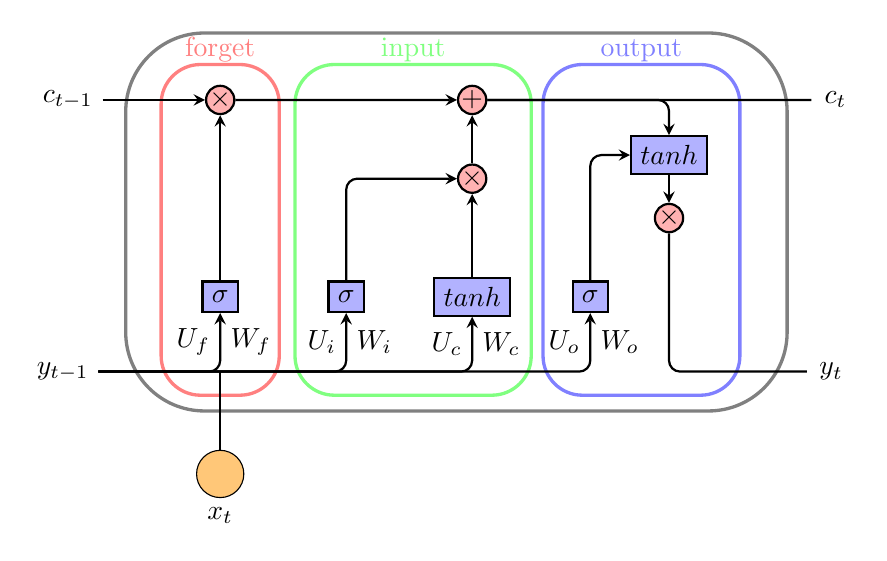
\begin{tikzpicture}

\node[draw=black, minimum width=6mm, circle, fill={rgb:orange,1;yellow,2;pink,5},label=270:$x_t$] (x) at (0,0) {};

\node[minimum width=6mm, left of=x, yshift=1.3cm, xshift=-1.0cm] (yt1) {$y_{t-1}$};



	\draw[-stealth, very thick, gray, above=2pt of x, rounded corners=10mm, yshift=0.8cm, xshift=-1.2cm] rectangle (8.4, 4.8);

	\draw[-stealth, very thick, red!50, above=2pt of x, rounded corners=5mm, yshift=1.0cm,xshift=-0.75cm] rectangle (1.5, 4.2) node[midway, above, yshift=2cm] {forget} ;

	\draw[-stealth, very thick, green!50, above=2pt of x, rounded corners=5mm, yshift=1.0cm,xshift=0.95cm] rectangle (3.0, 4.2) node[midway, above, yshift=2cm] {input};

\draw[-stealth, very thick, blue!50, right= of x, rounded corners=5mm, yshift=1.0cm,xshift=4.1cm] rectangle (2.5, 4.2) node[midway, above, yshift=2cm] {output};


\node[rectangle, draw, thick, above of= x, fill=blue!30, yshift=1.25cm] (sig1) {$\sigma$}; 

\node[rectangle, draw, thick, right of= sig1, fill=blue!30, xshift=0.6cm] (sig2) {$\sigma$}; 

\node[rectangle, draw, thick, right of= sig2, fill=blue!30, xshift=0.6cm] (tanh2) {$tanh$}; 

\node[circle, draw, thick, above of= tanh2, minimum width=0.1cm,yshift=0.5cm, fill=red!30, inner sep=0pt] (mul2) {$\times$}; 
 


\node[rectangle, draw, thick, right of= tanh2, fill=blue!30, xshift=0.5cm] (sig3) {$\sigma$}; 

\node[circle, draw, thick, above of= sig1, minimum width=0.1cm, fill=red!30, yshift =1.5cm,inner sep=0pt] (mul1) {$\times$}; 


\node[minimum width=6mm, left= of mul1, xshift=-0.3cm] (ct1)  {$c_{t-1}$};

\node[minimum width=6mm, right= of ct1, xshift=8cm] (ct)  {$c_{t}$};

\node[minimum width=6mm, right= of yt1, xshift=8cm] (yt)  {$y_{t}$};


\node[circle, draw, thick,above of=mul2,, minimum width=0.1cm, fill=red!30,inner sep=0pt] (add) {$+$}; 

\node[circle, draw, thick,right of=sig3,yshift=1.0cm, minimum width=0.1cm, fill=red!30,inner sep=0pt] (mul3) {$\times$}; 

\node[rectangle, draw, thick, above of= mul3, fill=blue!30,yshift=-0.2cm] (tanh3) {$tanh$}; 

\draw[thick,rounded corners,->,>=stealth] (yt1) -| node[left,pos=0.75] {$U_{f}$} node[right,pos=0.75] {$W_{f}$} (sig1.south);
\draw[thick,rounded corners,->,>=stealth] (yt1) -| node[left,pos=0.75] {$U_{i}$} node[right,pos=0.75] {$W_{i}$} (sig2.south);
\draw[thick,rounded corners,->,>=stealth] (yt1) -| node[left,pos=0.75] {$U_{c}$} node[right,pos=0.75] {$W_{c}$} (tanh2.south);
\draw[thick,rounded corners,->,>=stealth] (yt1) -| node[left,pos=0.75] {$U_{o}$} node[right,pos=0.75] {$W_{o}$} (sig3.south);

\draw[thick,rounded corners,->,>=stealth] (sig3.north) |- (tanh3.west);
\draw[thick,rounded corners,->,>=stealth] (add) -| (tanh3);

\draw[thick,rounded corners,->,>=stealth] (sig2.north) |- (mul2.west);
\draw[thick,->,>=stealth] (tanh2.north) -| (mul2.south);


\draw[thick,->,>=stealth] (sig1.north) -- (mul1.south);

\draw[thick,->,>=stealth] (ct1.east) -- (mul1.west);

\draw[thick,->,>=stealth] (mul1) -- (add);
\draw[thick,->,>=stealth] (mul2) -- (add);
\draw[thick,->,>=stealth] (tanh3) -- (mul3);
\draw[thick] (x) -- (0,1.29);
\draw[thick] (add) -- (ct);
\draw[thick,rounded corners] (mul3) |- (yt);


\end{tikzpicture}
\caption[Architecture of a Long Short Term Memory Cell]{Architecture of a Long Short Term Memory cell (LSTM) - in red is the \textbf{forget gate}, in green the \textbf{input gate} and in blue the \textbf{output gate} - matrices on the left of lines are applied to $y_{t-1}$ and the one on the right to $x_t$}
\label{fig:lstm}
\end{figure}


LSTMs block consists in a \textbf{memory cell}, an \textbf{input gate}, a \textbf{forget gate} and an \textbf{output gate}.
The \textbf{memory state} is a high dimensional state holding the information about past inputs and is updated according to its previous state and new inputs.
The \textbf{forget gate} will decide what information in the current memory state the block should keep or delete. This forgetting operating is done as follow:

\[f_t = \sigma(W_{f} x_t + U_{f} h_{t-1} + b_f)\]

This forgetting vector is then applied in an element-wise way to the memory cell in order to keep or delete information.

The \textbf{input gate} is deciding what information to add to the memory cell using two operations that are then multiplied together. The first one is applying a sigmoid function to the input in order to select from which part of the input the information will be added and the second is applying a hyperbolic tangente to determine the value added. Then this gate is added to the current memory state after the forget state has been applied:

\[i_t = \sigma(W_{i} x_t + U_{i} y_{t-1} + b_i) \circ \tanh(W_{c} x_t + U_{c} y_{t-1} + b_c)\]

The \textbf{output gate}, as its name implies, is finally deciding what is the output using the memory state and the current input. The input will choose what to output using a sigmoid and the memory state will decide the value by applying an hyperbolic tangente:

\[y_t = \sigma(W_{o} x_t + U_{o} y_{t-1} + b_o) \circ \tanh(c_t)\]

Therefore the main equation for the memory state is the following:

\[c_t = f_t \circ c_{t-1} + i_t \circ \tanh(W_{c} x_t + U_{c} y_{t-1} + b_c)\]

Bidirectional Long Short Term Memory (BLSTM) (\autoref{fig:blstm}) is a combination of two regular LSTMs reading the same input sequence in two opposite directions. The output of these two LSTM networks are then concatenated to form a BLSTM. Bidirectional Long Short Term Memory are very efficient when it comes to handle input sequences that are not only interpretable linearly from their first element to their last but also have a global complex context.


\begin{figure}[h]
\centering

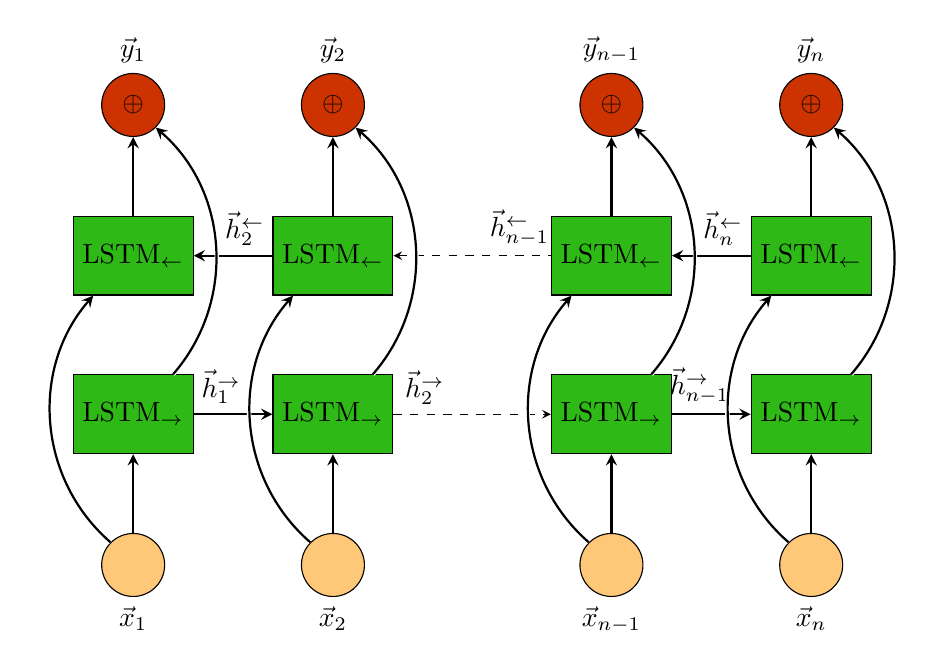
\begin{tikzpicture}

	\node[rectangle, draw, minimum height=1cm, minimum width=1cm,fill={rgb:red,1;green,4;blue,0.5}] (RNN) {LSTM$_\rightarrow$};
	\node[rectangle, right=of RNN, draw, minimum height=1cm, minimum width=1cm,fill={rgb:red,1;green,4;blue,0.5}] (RNN2) {LSTM$_\rightarrow$};
	\node[rectangle, right=2cm of RNN2, draw, minimum height=1cm, minimum width=1cm,fill={rgb:red,1;green,4;blue,0.5}] (RNN3) {LSTM$_\rightarrow$};
			
	\node[rectangle, right=of RNN3, draw, minimum height=1cm, minimum width=1cm,fill={rgb:red,1;green,4;blue,0.5}] (RNN4) {LSTM$_\rightarrow$};
			
			
	\node[rectangle, above=of RNN4, draw, minimum height=1cm, minimum width=1cm, fill={rgb:red,1;green,4;blue,0.5}] (R25) {LSTM$_\leftarrow$};
	\node[rectangle, left=of R25, minimum height=1cm, minimum width=1cm, draw,fill={rgb:red,1;green,4;blue,0.5}] (R24) {LSTM$_\leftarrow$};
	\node[rectangle, left=2cm of R24, draw, minimum height=1cm, minimum width=1cm,fill={rgb:red,1;green,4;blue,0.5}] (R23) {LSTM$_\leftarrow$};
	\node[rectangle, left=of R23, draw, minimum height=1cm, minimum width=1cm,fill={rgb:red,1;green,4;blue,0.5}] (R22) {LSTM$_\leftarrow$};
			
	\node[circle, draw=black, fill={rgb:orange,1;yellow,2;pink,5}, label=270:$\vec{x}_1$, minimum width=0.8cm, below=of RNN] (X1) {};
	\node[circle, draw=black, fill={rgb:orange,1;yellow,2;pink,5}, label=270:$\vec{x}_2$, minimum width=0.8cm,below=of RNN2] (X2) {};
	\node[circle, draw=black, fill={rgb:orange,1;yellow,2;pink,5}, label=270:$\vec{x}_{n-1}$, minimum width=0.8cm,below=of RNN3] (X3) {};
	\node[circle, draw=black, fill={rgb:orange,1;yellow,2;pink,5}, label=270:$\vec{x}_n$, minimum width=0.8cm,below=of RNN4] (X4) {};
	\node[circle, draw=black, fill={rgb:red,4;green,1;blue,0}, label=90:$\vec{y}_n$, minimum width=0.8cm,above=of R25] (Y5) {$\oplus$};
	\node[circle, draw=black, fill={rgb:red,4;green,1;blue,0}, label=90:$\vec{y}_{n-1}$, minimum width=0.8cm,above=of R24] (Y4) {$\oplus$};
	\node[circle, draw=black, fill={rgb:red,4;green,1;blue,0}, label=90:$\vec{y}_2$, minimum width=0.8cm,above=of R23] (Y3) {$\oplus$};
	\node[circle, draw=black, fill={rgb:red,4;green,1;blue,0}, label=90:$\vec{y}_1$, minimum width=0.8cm,above=of R22] (Y2) {$\oplus$};
			
	\draw[-stealth, thick] (X1) -- (RNN);
	\draw[-stealth, thick] (X2) -- (RNN2);
	\draw[-stealth, thick] (X3) -- (RNN3);
	\draw[-stealth, thick] (X4) -- (RNN4);
	\draw[-stealth, thick] (RNN) -- node[above, pos=0.35] {$\vec{h}_1^\rightarrow$} (RNN2);
	\draw[-stealth, dashed] (RNN2) -- node[above, pos=0.2] {$\vec{h}_2^\rightarrow$} (RNN3);
	\draw[-stealth, thick] (RNN3) -- node[above, pos=0.35] {$\vec{h}_{n-1}^\rightarrow$} (RNN4);
			
	\path[-stealth, ultra thick, white] (X1) edge[bend left=45] (R22);
	\path[-stealth, thick] (X1) edge[bend left=45] (R22);
	\path[-stealth, ultra thick, white] (X2) edge[bend left=45] (R23);
	\path[-stealth, thick] (X2) edge[bend left=45] (R23);
	\path[-stealth, ultra thick, white] (X3) edge[bend left=45] (R24);
	\path[-stealth, thick] (X3) edge[bend left=45] (R24);
	\path[-stealth, ultra thick, white] (X4) edge[bend left=45] (R25);
	\path[-stealth, thick] (X4) edge[bend left=45] (R25);
			
	\draw[-stealth, thick] (R22) -- (Y2);
	\draw[-stealth, thick] (R23) -- (Y3);
	\draw[-stealth, thick] (R24) -- (Y4);
	\draw[-stealth, thick] (R25) -- (Y5);
		
	\draw[stealth-, thick] (R22) -- node[above, pos=0.65] {$\vec{h}_2^\leftarrow$} (R23);
	\draw[stealth-, dashed] (R23) -- node[above, pos=0.8] {$\vec{h}_{n-1}^\leftarrow$} (R24);
	\draw[stealth-, thick] (R24) -- node[above, pos=0.65] {$\vec{h}_n^\leftarrow$} (R25);
			
	\path[-stealth, ultra thick, white] (RNN) edge[bend right=45] (Y2);
	\path[-stealth, thick] (RNN) edge[bend right=45] (Y2);
	\path[-stealth, ultra thick, white] (RNN2) edge[bend right=45] (Y3);
	\path[-stealth, thick] (RNN2) edge[bend right=45] (Y3);
	\path[-stealth, ultra thick, white] (RNN3) edge[bend right=45] (Y4);
	\path[-stealth, thick] (RNN3) edge[bend right=45] (Y4);
	\path[-stealth, ultra thick, white] (RNN4) edge[bend right=45] (Y5);
	\path[-stealth, thick] (RNN4) edge[bend right=45] (Y5);
			
\end{tikzpicture}
\caption[Example of a Bidirectional Long Short Term Memory network]{Bidirectional Long Short Term Memory network consists in two LSTM networks of opposite direction from which the outputs have been concatenated together.}
\label{fig:blstm}
\end{figure}

We will see in our study that stacked BLSTM layers are very efficient for handling structures such as spectrograms and extract useful information to operate source separation.

\subsection{Autoencoders and Sparsity}
\label{AE}

\begin{figure}[!hb]

\centering
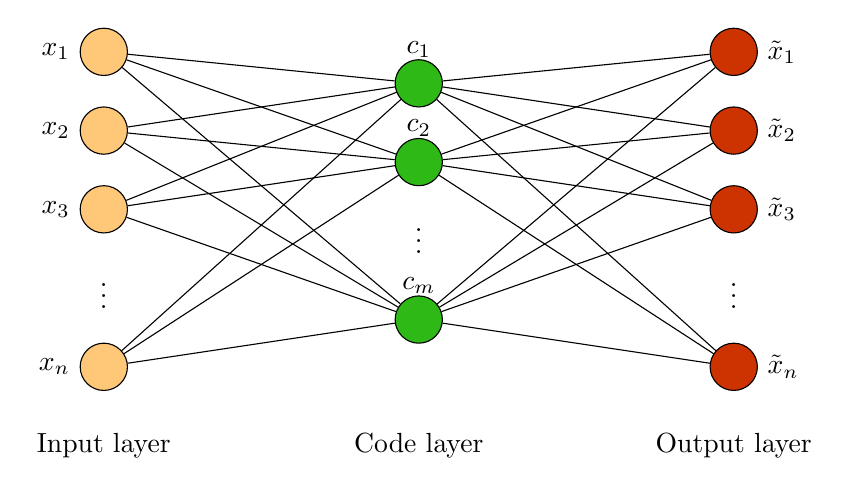
\begin{tikzpicture}

[   cnode/.style={draw=black,minimum width=10mm, circle}, ]
    \node at (0,-4) {$\vdots$};
    \node at (4,-3.3) {$\vdots$};
    \node at (8,-4) {$\vdots$};
    \node at (0,-6) {Input layer};
    \node at (4,-6) {Code layer};
    \node at (8,-6) {Output layer};
    \foreach \x in {1,...,4}
    {   
    \pgfmathparse{\x<4 ? \x : "n"}
        \node[draw=black, minimum width=6mm, circle, fill={rgb:orange,1;yellow,2;pink,5},label=180:$x_{\pgfmathresult}$] (x-\x) at (0,{-\x-div(\x,4)}) {};
    }
	
	 \foreach \x in {1,...,3}
    {
    \pgfmathparse{\x<3 ? \x : "m"}
        
        \node[draw=black, minimum width=6mm, circle,fill={rgb:red,1;green,4;blue,0.5},label={[label distance=0.1cm, yshift=-0.2cm] 90:$c_{\pgfmathresult}$}] 	(p-\x) at (4,{-0.4-1.0*\x-div(\x,3)}) {};
    }
    
    \foreach \x in {1,...,4}
    {
        \pgfmathparse{\x<4 ? \x : "n"}
        \node[draw=black, minimum width=6mm, circle, fill={rgb:red,4;green,1;blue,0},label=0:$\tilde x_{\pgfmathresult}$] (o-\x) at (8,{-\x-div(\x,4)}) {};
    }   
    
    
    
    \foreach \x in {1}
    {   \foreach \y in {1,...,3}
        {   
          \pgfmathparse{\y<3 ? \y : "m"}
        \draw (x-\x) -- (p-\y);
        }
    } 
    
    \foreach \x in {2,...,3}
    {   \foreach \y in {1,...,3}
        {   \draw (x-\x) -- (p-\y);
        }
    }
    
    \foreach \x in {4}
    {   \foreach \y in {1,...,3}
        {   
        \pgfmathparse{\y<3 ? \y : "m"}        
        \draw (x-\x) -- (p-\y);
        }
    }
    
    \foreach \x in {1,...,3}
    {   \foreach \y in {1,...,4}
        {   \draw (p-\x) -- (o-\y);
        }
    }
    
    
\end{tikzpicture}
\caption[Simple one-layered fully connected autoencoder]{Example of a one layer fully connected autoencoder. Here the coding layer has a smaller dimension than the input dimension.}
\label{fig:ae}
\end{figure}

Autoencoders \cite{AE}, also called auto-associators, are two layers perceptrons trained to reconstruct their input, and are in that sense called \textbf{self-supervised}. This particular architecture is trying to learn clever \textit{representation} of the input by reducing or increasing (overcomplete) the number of hidden units compared to this latter. This is done to avoid learning the identity function (what would happen if the hidden layer has the same size) and can force the network to learn specific features of the input in order to reconstruct it efficiently. Typically, with an input $x$, a two-layered autoencoder (\autoref{fig:ae}) is defined as:

\[
c(x) = f(W_1 \cdot x + b_1)
\]

\[
y = f(W_2 \cdot c + b_2)
\]

With $W$ and $b$ the weight and biases of the network, and $f$ the activation function. Here, $c$ is named the \textbf{latent representation},  the \textbf{code layer} or the \textbf{bottleneck} of the autoencoder, with $dim(c) < dim(x)$ or $dim(c) > dim(x)$, this hidden layer is the one learning interesting representations of the inputs. Then, once the autoencoder is trained to reconstruct its input, unsupervised algorithms such as k-means can be applied to cluster the dataset used to train the network.
Here we presented only a two-layered autoencoder but this architecture can certainly be extended to multiple layers and even use more complex operations such as convolutional or recurrent networks. Autoencoders are often divided in two main parts, the first one reducing the dimensionality of the input and the other one reconstructing it and increasing its dimensionality. They are often called the \textit{encoder} and the \textit{decoder}, or the \textbf{front-end} and the \textbf{back-end} of the autoencoder.

But shrinking or increasing the code layer size does not always suffice and other constraints have to be applied on the autoencoder in order to learn meaningful features.

With \textbf{denoising autoencoders}, inputs are corrupted with some random noise and the architecture is trained to learn their denoised version. The autoencoder is therefore forced to learn good features of the input but, as well to delete the noise added to this latter.

\textbf{Sparse autoencoders} are architectures where a \textbf{sparsity constraint} has been applied on the latent representation. \textbf{Sparsity} in the code layer implies that many units will be very close to the zero value and therefore units will be activated just to extract a very useful information for the reconstruction. For instance, an overcomplete autoencoder ($dim(c) > dim(x)$) without any sparsity constraint will be likely to learn similar features over the code layer or to converge to the identity function.

This constraint is added by forcing the latent units to have a small value $\rho$ in average. The activation value average of a code layer neuron over $n$ samples $(x^{(1)}, \dots, x^{(n)})$ can be computed by:

\[
\hat{\rho}_j = \frac{1}{n}\sum_{i=1}^n{c_j(x^{(i)})}
\]

Then, the sparsity constraint consist in imposing:

\[
\forall j,  \hat{\rho}_j = \rho
\]

To do so, a new term is added to the objective function of the autoencoder in order to maintain this equality. Commonly, the Kullback Leibler divergence is used to compare $\rho$ and $\rho_j$:

\[
L_{sparsity}(\theta) = \sum_{j=1}^{dim(c)}{D_{KL}(\rho||\hat{\rho}_j)} = \sum_{j=1}^{dim(c)}{\rho\log \frac{\rho}{\hat{\rho}_j}} + (1-\rho)\log \frac{1-\rho}{1-\hat{\rho}_j}
\]

The KL divergence can be seen as the measure of lost information when comparing two discrete probabilities, here every $\rho_j$ are approximating $\rho$.

In our study, the Adaptive layer presented in \autoref{adapt} is based on a sparse autoencoder structure.


\subsection{Loss function and Backpropagation}
\label{loss}
In order to train a neural network to learn a specific function in order to realize a specific task, it is needed to tell to the network '\textit{how much it is wrong}' in order to correct its next prediction. This is realized using an \textbf{objective function}/\textbf{loss function}/\textbf{cost function} which is telling the goal of our problem. This task can be seen as an optimization problem where the goal is to minimize or maximize the objective function in order to reach its global minimum or maximum point (depending on its definition) and thus reach the optimal solution. In order to reach this optimal goal associated with a particular objective with a deep neural networks the backpropagation algorithm coupled with the stochastic gradient descent algorithm.


The \textbf{backpropagation algorithm} \cite{BACKPROP} is the method used to compute the partial derivatives needed for the stochastic gradient descent algorithm. It is commonly said that the backpropagation step encompasses the gradient computation and the weights update of the neural network,but actually there are three distinct steps, (1) the forward step consisting in inputting the training samples and computing the neural network outputs, (2) the backpropagation computing the partial derivatives of the objective function and finally (3) the stochastic gradient descent algorithm is applied and all the weights are updated.

The backpropagation algorithm is using the \textbf{chain rule} in order to compute the gradient of the objective function $L(\theta; X)$ with respect to each weight $\theta_i$ (their \textit{influence} on the loss function) defined as $\frac{\partial L(\theta; X)}{\partial \theta_i}$. For instance, if $L(\theta; X) = h(\theta)$, using the chain rule, we can compute $\frac{\partial L(\theta)}{\partial \theta}$ as:
\[
\frac{\partial L(\theta)}{\partial \theta} = \frac{\partial L}{\partial h} \frac{\partial h}{\partial \theta}
\]

If the whole network is made of differentiable operations then it is possible to \textit{backpropagate} the gradient all along until the input layer and thus compute the influence of each weight and update them accordingly using the stochastic gradient descent formula:

 \[
\theta^t = \theta^{t-1} - \alpha \frac{\partial L(\theta^{t-1})}{\partial \theta}
 \]

The vanishing gradient problem by the sigmoid function mentioned in \autoref{ffn} is explained by the fact that during the training phase, bacpropagation algorithm is used and the minimum (which can be local) is searched iteratively in the opposite direction of the error derivative. During the backpropagation process, the sigmoid derivative function is used and multipled between each layers. The problem is that this function lies in $(0, 1/4]$ and these multiplications make the gradient vanish the more it backpropagates it.
Furthermore, because of this problem, the first layers of our Neural Network are slower to train than the last one and this might results in a huge inaccuracy at the end. For example in CNNs, as mentioned, first layers learn large features so that the next layers refined these features as much as it goes deeper. The vanishing gradient problem implies that the refined features will have in input corrupted information from the previous layers and therefore will not be able to learn useful patterns.

\subsection{Regularization}

One of the biggest problem that neural networks can encounter during its training phase is \textbf{overfitting}, meaning that it can predict very well on the training data but cannot generalize to new data (\autoref{fig:gen}). Regularization tries to solve this overfitting problem by penalizing the objective function with a certain additional term.

\begin{figure}[h]
\centering
\includegraphics[width=0.6\textwidth]{gen}
\caption[Generalization problem explanation]{We say there the network is \textbf{overfitting} the training set when the training error continues to decrease while the test error is increasing - Here the figure explains the concept of \textbf{early stopping} to counter the overfitting problem}
\label{fig:gen} 
\end{figure}



\[
L_{reg}(\theta; X, y) = L(\theta; X, y) + \lambda \Omega(\theta)
\]

Here, $\lambda$ is named the regularization coefficient and $\Omega(\theta)$ is some function contibuting positively on the objective function in order to penalize it with the parameters $\theta$. In this section we present several regularization functions and methods to decrease the generalization error.

The \textbf{$L_2$ regularization}, also known as the ridge regression in linear regression, constraints the network to be trained on small weights, and is defined as follow:

\[
\Omega(\theta)= \frac{1}{2}|| \omega ||^2_2
\]

The \textbf{$L_1$ regularization}, also known as the LASSO penalisation, tends to produce sparse weights in the neural network, meaning that many of them will be very close to the zero value:

\[
\Omega(\theta)= || \omega ||_1=\sum_i|\omega_i|
\]

\textbf{Dropout} \cite{DO} regularization method consists in removing randomly a hidden or visible unit in a neural network every step with the probability $p$. Dropping out units is done independently in each layer and at each step. This method can be seen as an \textit{ensemble learning} where each dropped out network learns data in its own way, with different errors, and in that way, by combining them averagely, this leads to a stronger architecture and avoids overfitting. At the test time the whole neurons of the network are used.

Another possible regularization during the training phase is to \textbf{increase the number of samples} in the dataset used. This can be done by generating new samples from the current dataset with some operations like flipping, rotating, clipping or adding noise.

One of the mostly commonly used and simple technique is called the \textbf{early stopping} (Explained in \autoref{fig:gen}). This approach consists in evaluating the network on a validation set during the training phase after a certain number of step, e.g. after every epoch. Overfitting can therefore be detected if the current validation set evaluation is higher than the previous one. Commonly, it is set to stop the training after a certain number of evaluations with a lower accuracy than the previous best one. 

In this study, early stopping is used to avoid overfitting, we set it so that the training phase stops when the validation set accuracy does not decrease anymore after 5 evaluations. In addition, recurrent dropout is used in the stacked BLSTM networks.

\subsection{Optimization}

During the optimization phase, three types of gradient descent exists. Firstly, the \textbf{batch gradient descent} is taking in input the whole dataset and then updating the weights accordindly. Using this method guarantees to converge to the global minimum for convex objective function and local minimum for non-convex one but this method is intractable for huge dataset which can not fit entirely in memory and is not able to handle online learning. The second method, named the \textbf{stochastic gradient descent} (SGD), consists in updating the weights after each sample has been fed to the network and is therefore way faster than the first one and can use online learning training. But there can be a huge variance between each update and thus the training phase becomes very noisy in terms of convergence. The third and today commonly used method is the \textbf{mini-batch gradient descent} which considers $n$ samples for updating the weights. Thus, the variance between each update is decreasing as much as the minibatch size increasesn but this size becomes a new hyperparameter to tune for training a neural network. This latter method is often called directly the SGD by misuse of language because minibatches are now universally used during the training phase.

In this section we present three main extensions for the Stochastic Gradient Descent: the momentum, RMSProp optimizer and Adam optimizer.
\subsubsection{Momentum}

One problem with the SGD method are ravines, surfaces where the curve is steeper in a direction than the other. Since SGD is pointing to the steepest direction rather than in the direction of the optimum, it will oscillate before reaching the surface minimum. Adding momentum helps the SGD to accelerate in ravine surfaces and is defined as follow:
\[v_t = \gamma v_{t-1} + \eta \nabla_\theta J(\theta)\]
\[\theta_t+1 = \theta_t - v_t\]
The momentum term $\gamma$ is commonly set to the value $0.9$. One extension to the Momentum method is the Nestorov Accelerated Gradient (NAG) [cite].
\subsubsection{RMSProp optimizer}
Root Mean Square Propagation (RMSProp) optimizer \cite{hinton2012neural} consists in exponentially decaying the learning rate using the average of squared gradients.
Defining $g_t = \nabla_{\theta_t}J(\theta_t)$ gradient of the loss function to the parameter $\theta_t$t, $\eta$ the initial learning rate, RMSProp method is defined as follow:

\[E[g^2]_t = 0.9E[g^2]_{t-1} +0.1g^2_t\]
\[\theta_{t+1} = \theta_t - \frac{\eta}{\sqrt{E[g^2]+\epsilon}} g_t\]

\subsubsection{Adam optimizer}


Adaptive Moment Estimation (Adam) optimizer \cite{ADAM} approach can be seen as an update of RMSProp where in addition to computing exponentially decaying squared gradient $v_t$, it considers as well the exponentially decaying gradients $m_t$ as follow:

\[m_t = \beta_1 m_{t-1} + (1-\beta_1)g_t\]
\[v_t = \beta_2 v_{t-1} + (1-\beta_2)g_t^2\]

Since it has been observed that $m_t$ and $v_t$ are biased for $\beta$ values close to 1, a bias correction is applied and:

\[\hat m_t = \frac{m_t}{1-\beta_1}\]
\[\hat v_t = \frac{v_t}{1-\beta_2}\]

Finally, we can see Adam optimization method as a combination of RMSProp and Momentum defined as:

\[\theta_{t+1} = \theta_t - \frac{\eta}{\sqrt{ \hat v_t}+\epsilon} \hat m_t\]

It has been shown (\autoref{fig:adam}) that Adam can lead to better results in terms of convergence than other optimizers.

\begin{figure}[h]
\centering
\includegraphics[width=0.6\textwidth]{adam}
\caption[Comparison of SGD, Adam and RMSProp performances]{ Adam Optimizer has better convergence than other optimizers such as RMSProp on the MNIST dataset with a multilayer neural network with dropout - Figure from Adam's paper \cite{ADAM}}
\label{fig:adam} 
\end{figure}

In our study, we use both RMSProp and Adam optimizers and select the one leading to the best accuracy. To do so we run the same experiments with different optimizers and learning rates.

\chapter{Related work}

In this chapter, we firstly discuss about the previous methods used to perform the multi speaker separation problem and secondly, since our study is mainly based on these works, we explain in more details both versions of Deep Clustering, the Source Contrastive Estimation and the Deep Attractor Network methods.

Firstly, \cite{Weintraub:1985:TCM:912498} and \cite{ GRAPS} are one of the very first works from M. Weintraub trying to separate two different speakers using Markov Models to infer binary masks. He introduced the GRAPS (Grouping Research on Auditory Sound Processing) method which uses onset and pitch features of speeches in order to extract useful information about the speakers and being able to separate them.
Following this work, Computational Auditory Scene Analysis systems (CASA) \cite{CASA1, CASA2} were introduced. They are systems extracting sounds components and are based on the biological inspiration from the Auditory Scene Analysis (ASA) \cite{ASA}. They try to reproduce source organization achieved by human beings using two main steps: the segmentation phase and grouping phase. Firstly, the segmentation phase extracts information such as harmonicity, pitch, coherent amplitude, or onsets, and then the grouping phase clusters features having similar characteristics to achieve the separation. But since these systems are mostly hand-crafted for the feature extraction they can not perform well on very noisy environments and therefore on real world application. 

Factorization models such as the Non Negative Matrix Factorization \cite{SNMF, NMFalgo} (NMF or NNMF) consist in learning in a supervised or unsupervised manner a good factorization of a learned dictionnary and activatons bases from spectrograms magnitudes. Then the learned bases can be used to separate the speaker voice they are associated to. But NMF methods are very costly and generate weak representation for the source separation problem. Moreover, NMF struggles to generalize to new environments and voices, it is more successful in structured signals like in music.
All theses previous methods did not have very good performances for the multi speaker separation problem because of they struggle generalizing to other speakers.

With its success in many areas like image processing, Deep Learning has recently been as well intensively applied in the audio processing domain. For instance, architectures such as WaveNet \cite{WaveNet} and more recently Tacotron 2 \cite{Tacotron2} have brought a huge leap in terms of performances compared to previous techniques in speech synthesis from text.

In the area of speech enhancement, which is closely related to source separation, fully connected networks \cite{DLSS}, stacked LSTM layers \cite{SELSTM, DAVSE}, deep stacked autoencoders \cite{AESE} and more recently residual networks (ResNet) coupled with visual information \cite{SpeechEnh} significantly improved the results in this domain in terms of Signal to Noise Ratio (SNR).

For the source separation problem, the first works involving deep neural networks tried to directly infer binary or soft masks using fully connected networks \cite{DNNSS, MASKDNN, MasksDNN, MASKDNN2}, CNN \cite{CNNrecog, Karaoke} and later networks such as stacked recurrent neural networks \cite{RNNSS, DNNSS2} and LSTM \cite{OverviewSSDL,LSTMSS, SpeechEnh} were used to perform this task. In \cite{AESS, AESS2} a unique  denoising autoencoder per source was trained to extract especially this latter. In addition, applying clustering algorithm on the latent representation of an autoencoder trained on spectrograms magnitudes of speakers mixtures did not lead to a good separation \cite{AESSsimple}. All these first methods have a drawback that is a bad generalization since they are all class-based  methods and therefore are good on the targets they were trained on. 

In the task of voice and music separation, \cite{Karaoke} is one of the first work infering masks to separate music and lyrics with CNN layers, later, \cite{chimera} using the Deep Clustering method coupled with direct mask inference significantly improved the results in this area.

Today's methods performing well in terms of SDR improvement for the single channel multi-speaker separation problem are deep learning architectures outputting discriminative embeddings for each TF-bins in order to be able to separate all the sources. Deep Clustering \cite{DPCLV1} is the first work introducing this method for the source separation problem, other other works such as Deep Attractor Network (DANet) \cite{DANet} and Source Contrastive Estimation (SCE) \cite{SCE} followed this approach. In parallel, Permutation Invariant Training (PIT) \cite{PIT, PIT1, PIT_recog} method used first CNN and now BLSTM layers to infer soft mask, compared to previous works directly inferring masks with such deep neural architectures, PIT is able to solve the permutation by considering all the possible permutation in output and is trained on the most probable match. 

Other works on the source separation problem  combines the use of audio mixtures and videos \cite{DAVSE, ImageSS, SpeechEnh}, and show that this additional visual information can lead to similar and even better results than previous methods. In particular, \cite{ImageSS} shows that the deep neural networks coupled with videos are mostly focusing their attention on the speaker mouth to identify who is speaking.


In \cite{TAS, Adaptive}, end-to-end non-linear architectures that are based on the autoencoder principle are applied directly on audio signals without using the STFT operation as preprocessing. 
The Adaptive layer presented in Section \ref{adapt} is mainly based on \cite{Adaptive} that shows that an autoencoder architecture can improve the source separation performance compared to the use of the audio mixtures Dicrete Cosine Transform as input.

\section{Deep Clustering (DPCL)}

Deep Clustering \cite{DPCLV1,DPCLV2, DPCLEXT, chimera} is one of the first method with a great accuracy on speech separation using deep learning architectures. The significant improvement of deep clustering compared to previous methods is that this approach is a partition-based segmentation algorithm in opposition to the previous class-based methods. Therefore, this method is really good at generalizing to other speakers where previous ones were struggling because only capable to decently handle examples there were trained on. The flexibility and good generalization brought by Deep Clustering is one of the reason of the leap it made in terms of SDR improvement compared to previous methods.

In this section, we explain in details how Deep Clustering can efficiently separate voices from a mixture and in a second phase we introduce its second version enhancing the results using some new methods on which our study will be in part based on.

\subsection{Discriminative Embeddings}
\label{DE}
Deep Clustering is using the spectrogram magnitude
These spectrograms are fed into a deep neural network that is outputting embeddings $V = f_\theta(x) \in \mathbb{R}^{T \times F \times E}$. With $E$ the size of the embedded space.
Beside theses embeddings, a target partition matrix $Y \in \mathbb{N}^{T \times F \times C}$ is created,  with $C$ designating the number of speaker in the input mixture. This matrix is defined so that $y(t,f)^{(c)} = 1$ if the speaker $i$ is dominant at the $(t,f)$ bin, $y(t,f)^{(c)} = 0$ otherwise, corresponding to the Ideal Binary Mask of the mixture. The affinity matrix $A = YY^{T}$ is then created and the estimated affinity matrix can be constructed with the inferred embeddings $V$ with $\hat{A}=VV^{T}$. The network is then trained such that $A$ equals $\hat{A}$ with the following cost function:
\[L_{DPCL}(\theta) = \norm{ A - \hat{A}}^2_F =  \norm{ YY^{T} - VV^{T}}^2_F \]
 
The deep neural architecture used in this study is a two stacked BLSTM of 600 hidden unit (300 units in each LSTM cell) with a feedforward neural network projecting the output in the embedded space of size $E$. This neural network is trained on the objective defined previously with spectrogram mixtures and the ideal binary mask used to construct the affinity matrix $YY^T$. Each generated embeddings by the deep neural architecture is unit normed.

During the inference phase, Deep Clustering method can solve the permutation problem using three different methods. The first one consists in giving in input the whole utterance to separate each source, in this case, k-means is used on the generated embeddings to create the partitions corresponding to each speaker. Secondly, instead of giving the whole mixture, like in the training, the embeddings are inferred on utterance chunks and k-means is applied on each chunk. But a permutation problem has to be solved in order to assure a continuity between each chunk, and to do so they compute the permutation giving the lowest $L^2$ distance between the whole separated spectrograms and the original one. In their paper, both method could deliver 
\subsection{End-to-end architecture}
\label{EEA}

As explained, the first version of Deep Clustering \cite{DPCLV1} approach constructs binary masks via the k-means algrithm applied on the embeddings to perform source separation. In their second paper \cite{DPCLV2}, they introduced an additional layer to transform these binary masks into soft masks and applied a soft differentiable version of k-means in order to finetune the whole network. The final network consists of the deep clustering part, the soft k-means and finally the enhancement layer.
Furthermore, they improved their architecture by adding regularization such as dropout and gradient normalization during the training phase. They have shown as well that using more stacked BLSTM with a smaller number of units inside each LSTM leads to better results.
In addition, they \textbf{pretrain} their network on small context window of size 100 and then finetuned it with a context window of 400. Finally, an end-to-end training was applied to finetune the whole network and led the best result they could obtain.

The enhancement layer consists in concatenating the separated spectrogram magnitudes with the spectrogram magnitude of the mixture along the frequency axis: $Y_j = [\tilde X_j, X] \in \mathbb{R}^{T\times 2F}, j \in [1\dots M]$.
 This tensor is fed to a BLSTM network followed by a feedforward neural network projecting the output on $z \in \mathbb{R}^{S\times TF}$. This output represents the new assignement for each separated speaker. A softmax function is then applied in order to output new soft masks $\tilde m_i$ in $[0,1]$:
\[
\tilde m_i = softmax(z)_i  = \frac{e^{z_i}}{\sum_j{e^{z_j}}} 
\]

Then these masks are applied on the mixture spectrogram to separate each source:

\[
x_i = m_i \cdot X
\]

\textbf{TODO : Loss}

We implement this layer to first reproduce the results of DPCL \cite{DPCLV2} and secondly to apply it to the SCE method in order to enhance its results.

\section{Source Contrastive Estimation (SCE)}

The Source Contrastive Estimation method (SCE) \cite{SCE} is based on the same approach than Deep Clustering consisting in generating contrastive embeddings in order to apply clustering, create masks and separate all the sources. This method is based on the \textit{word2vec} work.
Instead of learning to approximate the affinity matrix $A = YY^{T}$, the Source Contrastive Method applies a stronger constraint on the generated embeddings. \textbf{TODO : details}

\[L(\theta) = - \frac{1}{M} \sum_{t,f} \sum_{s} \log \sigma(Y_{t,f}^{(s)} \cdot v_i(t,f)^{T} v_o^{(s)})\]

This loss function tends to pull together embeddings and speaker vector from the same speaker and on the contrary tends to push away the one not belonging to a specific speaker.


\section{Deep Attractor Network (DANet)}


Introduction to DAnet approach

Difference with DPCL and SCE

Loss function

\[a_s = \frac{\sum_{t,f}{Y_{(t,f)}^{(s)}V_{t,f} }}{\sum_{t,f}{Y_{(t,f)}^{(s)}}} = \frac{{Y_s^TV}}{\sum_{t,f}{Y_{(t,f)}^{(s)}}}\]

\[d_s = a_sV, s = 1,..., M \]
\[\tilde{m_s} = f(d_s)\]

\[L_\theta(x) = \frac{1}{M} \norm{x \cdot (m_i - \tilde{m_j})}^2_2 \]

In their paper, the authors propose two approaches during inference phase for the DANet architecture. The first one is ,like in the previous methods presented, using K-Means algorithm in order to generate masks and separate each speaker voice. The second one consists in using fixed attractors that are chosen using the centroids returned by K-Means algorithm.

\chapter{Experiments}

\section{Environment}

The framework used for all our deep learning architecture is TensorFlow r1.9 \cite{TF} and the experiments were conducted using RAIDEN Computer System provided by RIKEN AIP. This system has nodes with NVIDIA DGX 100 composed of 8 Nvidia Tesla V100-SXM2-16GB of 15GB of RAM. Our experiments were computed on a single GPU but our implementation makes them runnable on multiple GPUs. 

To evaluate our experiments in terms of Signal to Distortion Ratio (SDR) and Signal to Interference Ratio (SIR) improvements, we used the BSS\_EVAL toolbox \cite{BSS}. Since we are working on NVIDIA DGX 100, and that these later are shared among RAIDEN users GPU, using the BSS\_EVAL Python module on CPU can be  very slow when the CPU shared. Therefore, to speed-up the testing phase, we implemented the BSS\_EVAL toolbox with CuPy \cite{cupy} and TensorFlow r1.9 in order to run all the experiments fully on GPUs - note that this new implementation is only compatible with TensorFlow r1.9, which is the first version capable of handling \textit{complex128} numbers for the $FFT$ operation and therefore having good enough precision to deliver similar results as the original CPU-version module

\section{LibriSpeech ASR Corpus and optimization}

For all the experiments conducted in our study we used the LibriSpeech ASR Corpus \cite{LIBRI}. From this dataset, we used the \textit{train-clean-100} set containing 100 hours of 125 women and 126 men speeches. This dataset was split in three parts: the training representing 80\%, the validation 10\% and the test 20\% set. Another set was created with \textit{test-other-clean} to evaluate our models on \textit{out-of-set} speaker mixtures. For computational speed up and memory savings we downsampled the audio signals from 16kHz to 8kHz.
When spectrograms are used as input, we computed the Short Time Fourier spectral magnitudes for each mixture with a window size of 32 ms (256 samples), a hop size of 8 ms (64 samples) with the square root of the Hann as window. From these spectrograms were build the ideal binary masks $Y$ by evaluating the dominant speaker for each $(t,f)$ bin.

In our implementation, we do not precompute the spectrogram magnitudes and store them like it is usually done. We directly use the raw audio files as inputs because our models have to be able to compare their results on the same audio files using the Adaptive layer or spectrogram magnitudes. To do so, we stored the audio signals in \textit{.tfrecords} files that are processed by the \textit{tf.data.Dataset} API. Using directly the TensorFlow format file and API for data importation enables the use of operations such as \textit{tf.data.map} allowing the manipulation of audio files on multiple processes and \textit{tf.data.prefetch} which is prefetching next batches on the CPU while the previous one are computed on the GPU.
All these optimized operations for the input data generation leads to a significant speed-up for large batches of 256 elements. A good advantage of this method is that it can randomly generate many different mixtures with different chunk sizes, number of speakers and genders without to have to store the inputs on the hard disk - random states are set constant during the training phase in order to have reproducible results. But one drawback is that it is computing exactly the same inputs every epochs and therefore can be seen as quite time consuming.
 Furthermore, since the non-chunked raw data are stored, our implementation is capable to generate chunked mixtures of different size and therefore can generate. All our code can be found at \cite{github}.

\chapter{Contributions}

In this chapter we present in more detail the contributions mentioned in \ref{contrib}. Firstly, we describe the architecture we use to replace the use of spectrogram magnitude as inputs and that we use with Deep Clustering and Source Contrastive Estimation. Secondly, we describe the improvements we propose for the SCE method, such as using a soft version of k-means, negative sampling, a silent loss function and other approaches brought by \cite{DPCLV2}, the second version of Deep Clustering.

\section{The Adaptive Layer}
\label{adapt}

The main idea in this section is based on an end-to-end architecture presented in \cite{Adaptive}. This work shows that the use of a non linear autoencoder directly on audio mixture can lead to better performances than using the DCT of these latter. This autoencoder consists in two main parts, as explained in Section \ref{AE}, a front-end creating a latent representation of the input and a back-end reconstruction the input.

Our idea is to apply such an approach to the current deep learning state of the art methods - in this study DPCL and SCE - in order to see if this method can lead to any improvement.
 
First of all, since Deep Clustering and Source Constrastive Estimation methods are not trained in an end-to-end way, meaning that the output of the network during the training phase does not lead to the reconstruction of the separated signals, then it is impossible to simply add such an architecture '\textit{around}' the deep neural architectures and train it as a whole. In fact, if we want to train one of these methods using an autoencoder, then only its front-end part can be plug on since the network does not output separated inputs and therefore the autoencoder can not be trained during the training phase of these two methods. Moreover, if only the front-end is used during the training phase then the latent representation will not have any sense in terms of feature extraction since the reconstruction phase is absent. 

The solution we propose consists in pretraining the autoencoder for the multi-speaker separation problem. The main difference with standard autoencoders is that in this case we do not train to reconstruct the input but to reconstruct the separated signals. To do so, the autoencoder is \textbf{(1)} fed with a \textbf{mixture of signals and the original signals from this mixture}, then \textbf{(2)} computes the separation and \textbf{(3)} reconstructs each separated signals.

To perform these three operations, we present a \textbf{sparse linear autoencoder} consisting of a front-end layer, a separation operation and a back-end layer. The front-end layer is a one-dimensional convolution operation and a max-pooling layer and the back-end layer is composed by an unpooling and a deconvolution layer.

\textbf{Front-end layer}
As mentioned, the input consists in a audio mixture $x = \sum_{j=1}^{M}{x_j} \in \mathbb{R}^L$ with the original signals $x_j \in \mathbb{R}^L$, $M$ being the number of mixed signals. We name $X$ the output of the front-end layer corresponding to $x$ and $X_j$ the outputs corresponding to the original signals $x_j$. Since we want to perform a quasi perfect separation between the encoder and the decoder, the front-end layer must be as linear as possible. Indeed, if the linearity is lost by this latter $X \simeq \sum_{j=1}^{M}{X_j}$ does not hold and therefore it is not possible to apply filters in order to separate each signal.
The front-end we define is composed of two operations. The first one is a \textbf{one-dimensional convolution operation} applied on the inputs as follow:

\[Y = 1DConv(x) = W_{f} \ast x = (|\omega| \cdot B) \ast x\]

With $W_f \in \mathbb{R}^{F\times N}$ the $F$ convolution filters of size $N$ applied along the time axis. Here, this matrix is more specifically defined as $W_f = |\omega|\cdot B$ with $\omega \in \mathbb{R}^{N}$ representing the window whereas $B \in \mathbb{R}^{F\times N}$ represents the bases of the operation.

This convolution layer is followed by a \textbf{maxpooling operation} along the time axis with a stride and hop of size $m$:

\[X = maxpool(Y, m)\]

This maxpooling layer is a non-linear operation but for $M = 2$, we can suppose that $X \simeq \sum_{j=1}^{M}{X_j}$. We will see in Section \ref{adapt} that the maxpooling operation in the Adaptive layer is indeed a drawback for the reconstruction for $M > 2$ but that this operation is necessary to have a decent sparsity in the latent representation.

\textbf{Separation:} Once the encoder outputs are computed it is possible to separate the mixture representation using the original separated signals representation. For instance, $m_j$ is the mask extracting the $j^{th}$ original signal and is computed as:

\[m_j = \frac{X_j}{\sum_j{X_j} + \epsilon} \simeq  \frac{X_j}{X + \epsilon}\]

The it suffices to apply these masks on the mixture representation to have the separated signals:

\[\tilde X _j = m_j \cdot X\]

\textbf{Back-end layer:} The decoder is processing the separated latent representations to reconstruct the original signals. First, it applies an unpooling and then a deconvolution operation. The unpooling operation we use is following the method proposed in \cite{unpool} that is putting the values where the maximum values were computed by the maxpooling of the front-end, with zeros anywhere else. This method presents better results than gathering the values at the up-left corner of each unpooled patches because it is structurally preserving information. Then, the deconvolution layer has the structure as the front-end convolution but does not share the same weights. We name the reconstructed separated signals $\tilde x _j$

\textbf{Objective function}: To train our autoencoder we are using the Mean Square Error (MSE) loss with a sparsity constraint and an additional loss that we name the \textit{overlapping} loss:

\[L_\theta(x) = \frac{1}{M}\sum_{j=1}^{M}{\norm{x_j - \tilde{x}_j}}^2 + \beta KL(\rho, \hat{\rho}) + \alpha \cdot overlapping(x)\]

The overlapping loss function is added in order to reduce the overlapped number of information and therefore push out model to learn good bases functions to distinguish well each signals. This loss is comparing each couples of the sparse representations generated by the front-end layer (without considering the one involving the mixture of all the signals). For a couple $(X_1,X_2)$
\[overlapping(X1, X2) = \] 

In Section \ref{adapt}, we present the results with different hyperparameters for the pretraining phase of the Adaptive layer. Then we apply the pretrained front-end to DPCL and SCE to train these deep neural networks and we finally plug the back-end layer to finetune the whole network. But to be able to finetune the whole network, the clustering operation must be differentiable.

\section{Soft K-Means implementation}

As explained in Section \ref{EEA}, the second version Deep Clustering used a soft version of k-means in order to be able to apply backpropagation on the whole network and therefore being able to finetune it in an end-to-end way. In this section we will explain what this soft k-means algorithm consists in and how we implemented it efficiently on the TensorFlow framework.

The idea of using a soft version of k-means is to first be able to apply backpropagation on the whole network since the $argmax$ function used in the hard version is not differentiable and secondly, to produce softer masks and thus improve the separation. 

Let's consider the separation of $L$ points $x \in \mathbb{R}^E$ in $K$ clusters. Firstly, it consists in computing the soft assignment $\gamma$ of each point of the dataset to the centroids $\mu \in \mathbb{R}^{K\times E}$ that are randomly initialized. The assignment of the $i^{th}$ element to the $c^{th}$ cluster is defined as:

\[ \gamma_{i,c} = \frac{e^{-\beta |v_i-\mu_c|^2}}{\sum_{c^\prime} e^{-\beta |v_i-\mu_c^\prime|^2}}  \]

Then each centroid is updated as being the average sum of the point assignements

\[ \mu_c = \frac{\sum_i \gamma_{i,c}w_iv_i}{\sum_i \gamma_{i,c}}  \]


This algorithm can actually be interpreted as an Expectation Maximization (EM) with Gaussian Mixture Models (GMM) with a common shared variance. Indeed, a Gaussian Mixture Model is a weighted linear combination of gaussians and is defined as follow:

\[
 p(x | \mathbf{\mu}, \mathbf{\sigma}) = \sum_{i=0}^K \pi_i N(x, \mu_i,\sigma_i)
\]

With:

\[
N(x, \mu_i,\sigma_i) = \frac{1}{\sigma_i \sqrt{2\pi}} e^{\frac{(x-\mu_i)^2}{\sigma_i^2}}
\]

The first step of the EM method is the expectation step which compute the probabilities for each to point to each gaussian in the mixture, $p(k|x)$ that is the prior probabilities. This step computes what is called the \textit{responsibility}, i.e. how much each gaussian is responsible for each data. The responsabilities correspond to the assignements and are computed using the Bayes rule:

\[
\gamma_i(x) = p(i|x) = \frac{p(i)p(x|i)}{p(x)} = \frac{\pi_i N(x, \mu_k,\sigma_k)}{\sum_j \pi_j N(x, \mu_j,\sigma_j)}
\]

We can see that if we consider this mixture as being non weighted and having a shared variance then we obtain:

\[
\gamma_i(x) = \frac{N(x, \mu_k,\sigma)}{\sum_j N(x, \mu_j,\sigma)} = \frac{e^{\frac{(x-\mu_i)^2}{\sigma^2}}}{\sum_j e^{\frac{(x-\mu_j)^2}{\sigma_i^2}}} 
\]



Here $\beta$ is named the \textit{stiffness} and can be seen as the inverse variance of the Gaussian Mixture Models. Therefore, if $\beta$ is small the gaussian variance will be large and each point will have a higher degree of assignement, in the contrary, for large values the gaussians are narrow and the algorithm is close to its hard version.
\textbf{TODO}
\textbf{Graph with different beta - TODO}

Implementing hard k-means and soft k-means with TensorFlow presented several challenges. First, our version has to be able to handle the whole minibatch of embeddings $V\in R^{B\times TF \times E}$. Indeed, if k-means is applied iteratively on each sample of embeddings this would require a high amount of time and since an unique GPU is used, these operations can not be run in parallel. Therefore, in order to speed up the training time, our implemention is computing hard and soft k-means for a batch of data, at the same time. There was no necessary trick needed for the soft version since assignements and the centroids updates formulas can be extended to batches using tensors multiplications. Whereas with the hard version the assignements designate only one particular cluster, and to compute $\sum_i x[i = c]$ during the centroids update, the function \textit{tf.unsorted\_segment\_sum} is used to sum the vectors belonging to the same cluster. But , the solution is to shift the cluster assignement for each batch as follow:
\textbf{TODO}

Secondly, we implemented as well the use of several tries in order to avoid bad centroids initialization and thus improve the accuracy of our algorithm. To do so, we repeat the input $T$ times along its first dimension in order to have $V\in R^{T \times B\times TF \times E}$, i.e. $T$ tries of $B$ batches of $TF$ vectors of dimension $E$. Seeing these $T$ tries of $B$ batches as $TB$ batches instead reduces this problem to the first one. Once the $TB$ batches are clustered and that the $\mu \in R^{TB\times K \times E}$ centroids are computed by the algorithm, for each batch $b$ the argument with minimum inertia among its tries is selected as the actual clusters to output.

We show in Section \ref{softkmeans} that using soft k-means for the SCE method increases the SDR improvement, but sometimes to the detriment of the SIR improvement.



\section{Combining DANet and SCE methods}

One drawback of the Source Contrastive Loss function is its \textbf{locality}, because it is trained on each $(t,f)$ bins without being aware of the global context. For DANet, it is the contrary, it focuses on the globality of the context window by using weighted average vectors of generated discriminative embeddings and do not consider close relation between each embedded vector.
Our approach is to consider both methods at the same time in order to apply local loss function with the SCE loss and giving more context by adding the DANet loss function.

The loss function used for such network is therefore:

\[L(\theta) = L_{SCE}(\theta) + L_{DANet}(\theta)\]
\[L(\theta) = - \frac{1}{M} \sum_{t,f} \sum_{s} \log \sigma(Y_{t,f}^{(s)} \cdot v_i(t,f)^{T} v_o^{(s)}) + \frac{1}{M} \norm{x \cdot (m_i - \tilde{m_j})}^2_2\]

We show in Section~\ref{DANET} that this approach is leading to better results for a mixture of 2 speakers of different and same gender.


\section{Negative Sampling for Source Contrastive Estimation}

For the Source Contrastive Estimation method, training to separate two different genders is quite an easy task regarding the speakers embedded vectors since they only have to form two main clusters to correctly learn the difference between male and female speakers. But separating voice from the same gender and two different genders is more challenging since in this case not only two clusters have to be learnt but the number of speakers in the set. For instance, in our case, the LibriSpeech Corpus with 100 hours of speech contains 251 speakers (126 males and 125 females), thus to learn how to separate all possible of mixtures, the training phase has to study the relation between $\left(\! \begin{array}{c} 251 \\ 2 \end{array} \!\right) = $ couples. This is a very high number of couples to study and it might be impossible to have in input all the possible couples many times, even with a huge dataset generation. As we can see on Figure [CITE], learning with the loss [CITE] on a mixture of 2 speakers with same and different genders leads to a speaker vectors embedded space forming a 'ring'. This repartition leads to areas with bad male/male, female/female contrasts but even male/female in the area between both main male and female clusters. 

To tackle this problem, we propose to use \textit{Negative Sampling} method in order to extend the number of couples encountered during the training phase. This method is inspired from NEG objective function  defined in \cite{NS} where \textit{k} negative samples are drawn from a certain distribution. 

In our case, the general approach consists in selecting, for a $(t,f)$ bin, $v_o^{(k)}, k \in 1,\dotsc,K$ speaker vectors different from the dominant speaker vector $v_{o_{+}}(t,f)$ at this specific bin. In other words, $v_o^{(k)} \in V_o^-(t,f) = V_o/_{v_o^+(t,f)}$, and we define $\mathfrak{B}(t,f) = \{v_o^{(k)}, k \in 1,\dotsc,K\}$ the $K$ sampled vectors at a $(t,f)$ bin. We define the new loss function applying Negative Sampling for SCE as follow:

%\[L_\theta(x)_{NS} = - \frac{1}{M} \sum_{t,f} \sum_{s} \log \sigma(Y_{t,f}^{(s)} \cdot v_i(t,f)^{T} v_o^{(s)}) - \beta \frac{1}{K} \sum_{t,f} \sum_{v_o^{(s)} \in \mathfrak{B}(t,f)} \log \sigma(- v_i(t,f)^{T} v_o^{(s)}) \]

\[L_{NS}(\theta) = L_{SCE}(\theta) - \beta \frac{1}{K} \sum_{t,f} \sum_{v_o^{(s)} \in \mathfrak{B}(t,f)} \log \sigma(- v_i(t,f)^{T} v_o^{(s)}) \]

The first term corresponds to the objective function defined in [CITE] and the second one the added Negative Sampling. In this term $Y_{t,f}^{(s)} = -1$ since we want the $K$ selected vectors to be \textit{pushed away} from the dominant speaker vector, and this is apply for each $v_i(t,f)$ embeddings. The negative sampling term is multiplied by a coefficient $\beta \in[0,1]$ in order to give priority to the first term since it is the main objective function. Indeed, these two members have both the same magnitude: for instance, choosing $\beta = 1$ would lead to an equivalence in terms of influence for the SCE loss and Negative Sampling loss, and thus, the network would struggle learning the constrast between each speaker vectors because the Negative Sampling term would add too much noisy information to the SCE loss. 

In addition, we introduce two approaches to define $\mathfrak{B}(t,f)$. The first one consists in randomly selecting $K$ other speaker vectors from $V_o^-(t,f)$. This approach is randomly pushing away $K$ other speaker vectors of the embedded space, and therefore will cover all the possible different couples many times during the training phase:

\[\mathfrak{B}(t,f) = \mathfrak{B}_{rand}(t,f) = \{v_o^{(X_k)} \in V_{o_{-1}}(t,f) | X_k \in \mathcal{U}(1,|S|), k \in 1, \dotsc,K\} \]

The second approach consists in selecting the K-Nearest Neighbors (KNN) vectors of $v_{o_{+}}(t,f)$ and move them away for it. This idea is based on the local bad contrast obtained between speaker vectors of the same gender and tends to a more spread out speaker vectors embedded space:


\[\mathfrak{B}(t,f) = \mathfrak{B}_{KNN}(t,f) = \{v_o^{(i)} | \norm{v_{{(1)}}-v_o{_{+}}(t,f)} \leq \dots \leq \norm{v_{{(K)}}-v_o{_{+}}(t,f)}, i \in 1, \dotsc,K\}\]

In Section [cite] we show the performances of this approach with different values for $K$ and $\beta$. We try this method with spectrograms magnitude and the Adaptive Layer.


\section{General improvements of Source Contrastive Estimation}

\subsection{Source Contrastive Estimation Silenced Loss}

One drawback, we observed with the SCE objective function is that it is taking into account all the TF-bins embeddings $V \in R^{TF\times E}$ outputted by the neural network. The problem is that some of these TF-bins have very low energy and therefore are not very relevant since they don't hold much information about any specific speaker. Considering these almost silent bins is leading to a noisy training because some speaker embeddings will be equally trained on these noisy vectors and on the others holding much more information. Our solution implies to apply a mask on the loss function to omit these almost silent bins, as following:

\[L(\theta) = - \frac{1}{M} \sum_{t,f} \sum_{s} \log \sigma(W_{t,f}Y_{t,f}^{(s)}  \cdot v_i(t,f)^{T} v_o^{(s)})\]

The silent mask $W$ is omitting bins that are higher than a certain level $\tau$ of difference in decibel with the highest energy bin of the whole spectrogram:

$$
W_{t,f} =  \left\{
    \begin{array}{ll}
        1 & \mbox{if } 10\log (\frac{|X_{t,f}|}{max(|X|)}) < \tau \mbox{ in } dB  \\
        0 & \mbox{else}
    \end{array}
\right.
$$

In Section \ref{silentloss}, we show that using this silent mask is significantly improving SCE results with both spectrograms and the Adaptive layer.

\subsection{Pretraining, Enhancing and Finetuning}

Like in [], we first train the SCE on spectrograms or outputs of the Adaptive front-end with a certain chunk size and then continue to train the network on a bigger chunk size in order to improve its performance. This method can be seen as \textit{finetuning} the network on longer chunk size. Furthermore, being more accurate on longer chunk will with high probabilty improve the performance of our model, indeed during the test phase audio mixtures are chunked with the size the network has been trained on, for small chunk size it is more likely to have a high percenatge of silent area for the speakers and thus a quite noisy sample with few information to produce a good separation, whereas for longer chunks more information to be able to distinguish them is available.
Moreover, after the network has been fully trained on bigger chunks the enhance layer is added to SCE network in order to generate softer and better masks.And finally, since soft k-means is used we can finetune the whole architecture and see if this can lead to any further improvements.

We show in Sections \ref{ext}, \ref{enh} and \ref{finetuning} that these addings are indeed enhancing all methods in terms of SDR and SIR improvements.


\chapter{Results}
\label{res}

In this chapter we present our results on the environment and dataset presented in [CITE].
In the first section, using the LibriSpeech Corpus, we reproduce the results of the Deep Clustering and Source Constrastive Estimation methods. In the second section, we show our results using the Adaptive layer with these two methods: to do so we first analyze the \textit{pretraining} phase of the Adaptive layer for different hyperparameters and show some drawbacks encountered with this latter. In the third section we try all the contributions mentioned previously and see the improvements we could get.

For all the evaluations shown in this chapter, the models were evaluated on the chunk size they were trained on. To generate our test set we apply the procedure mentioned in [CITE EXP].
 
\section{State of the art results reproduction}

\begin{table}[ht]
\centering
\begin{tabular}{c|c|c|c|c|c|c}
\multirow{2}{*}{Improvements in dB} & \multicolumn{2}{c|}{m+m} & \multicolumn{2}{c|}{m+f} & \multicolumn{2}{c}{all} \\ 
\cline{2-7} 
 & SDR & SIR & SDR & SIR & SDR & SIR \\ 
\hline 
DPCL \cite{DPCLV1} & 4.00 &  & 9.07 &  & 6.54 &  \\ 
DPCL (ours) & 2.71 & 6.90 & 8.00 & 14.91 & 5.49 & 9.85 
\\ 
\hline 
\hline 
DPCL - enh (ours) & 6.79 & 11.47 & 10.14 & 16.09 & 7.59 & 12.34 \\ 
DPCL - ext (ours) & 3.21 & 7.20 & 10.43 & 17.97 & 4.74 & 9.28 \\ 
DPCL - ext + enh (ours) & 7.92 & 13.47 & 12.38 & 19.18 & 9.08 & 14.38 \\ 
\hline 
\hline 
DPCL++ \cite{DPCLV2} & 9.40 &  & 12.0 &  & 10.08 &  \\ 
DPCL - finetuned (ours) & - & - & - & - & - & - \\ 
\end{tabular}
\captionsetup{justification=centering}
\caption{Deep Clustering results reproduction}
\label{table:DPCLreprod}
\end{table}

\textbf{Deep Clustering:} In Table \ref{table:DPCLreprod} we report our results for the reproduction of the Deep Clustering approach. We can see that for the DPCL++ \cite{DPCLV2} approach we could reproduce the results (equivalent to \textit{DPCL - ext + enh (ours)}) but we could not have the same for its first version DPCL \cite{DPCLV1} (equivalent to \textit{DPCL (ours)}). This might be due to some hyperparameters difference, implementation, training time and type of data.

\begin{table}[ht]
\centering
\begin{tabular}{c|c|c|c|c|c|c}
DPCL chunk 100 & \multicolumn{2}{c|}{m+m} & \multicolumn{2}{c|}{m+f} & \multicolumn{2}{c}{all} \\ 
\hline 
k-means $\beta$ - silence & SDR & SIR & SDR & SIR & SDR & SIR \\ 
\hline 
hard $dB$ & 2.85 & 8.71 & 8.03 & 14.80 & 5.30 & 11.40 \\ 
hard - 20 $dB$ & 3.58 & 10.78 & 8.00 & 14.91 & \textit{5.49} & \textit{12.39} \\ 
\hline 
\hline 
5 - 20 $dB$ & 1.58 & 2.86 & 6.22 & 9.26 & 2.97 & 4.49 \\ 
10 - 20 $dB$ &  \cellcolor{green}\textbf{2.71} & \cellcolor{green}6.90 & \cellcolor{green}\textbf{8.42} &\cellcolor{green} 14.49 & \cellcolor{green}\textbf{5.12} & \cellcolor{green}9.85 \\ 
15 - 20 $dB$ & 1.82 & 7.23 & 8.34 & 14.88 & 4.51 & \textbf{10.15} \\ 
20 - 20 $dB$ & 1.60 & 7.25 & 8.22 & \textbf{14.93} & 4.25 & 10.11 \\ 
25 - 20 $dB$ & 1.53 & \textbf{7.27} & 8.13 & 14.92 & 4.13 & 10.08 \\ 
\end{tabular}
\captionsetup{justification=centering}
\caption{Evaluation of a Deep Clustering architecture (4x600) with different hyperparameters for kmeans and different type of mixture with 2 speakers - green cells are the parameters used for the next phase}
\label{table:DPCLV1}
\end{table}

From now on, we detail the process we followed from reproducing DPCL \cite{DPCLV1} to DPCL++ \cite{DPCLV2} results.
To reproduce the DPCL results we used an architecture consisting in 4 BLSTM layers of 600 units (corresponding to 300 units in each LSTM cell) with an embedded space of size $E=40$ - this size is set as constant for all the following experiments. This network is one BLSTM layer larger than the one used in \cite{DPCLV1}, but we see in the Table \ref{table:DPCLV1} that even using a larger network does not lead to the same results. In addition, instead of using a fully connected network as the final layer of our network, we replaced it by a one dimensional convolutional network, this is often leading to the same results and reduces the number of weights that can be high if the BLSTM units number or the embedded space size increases. Concerning the optimization, we use the RMSProp optimizer (\ref{RMS}) with a learning rate of $1e^{-3}$ that is halved every 50 epochs. We compare the SDR and SIR improvements using a regular hard version of k-means with and without silence and the soft version with different stiffness $\beta$ and a threshold of $20dB$. As regularization,as in DPCL++ \cite{DPCLV2}, in each BLSTM is  recurrent dropout and a gradient normalization of $200$ is used during the optimization phase.
These experiments are computed during 100 epochs using early stopping if the validation set accuracy does not decrease after 5 evaluations.
In many experiments results, it can be observed that with higher values of $\beta$ (harder stiffness) for the soft k-means algorithm, the SIR improvement is increasing, this is explain by the fact that the separation is \textit{stronger} (close to binary masks), there is less remaining of other sources in the separated one, and therefore less interferences, what SIR is actually measuring.

\begin{table}[h]
\centering
\begin{tabular}{c|c|c|c|c|c|c|c}
\multicolumn{2}{c|}{DPCL chunk 100 - enhance} & \multicolumn{2}{c|}{m+m} & \multicolumn{2}{c|}{m+f} & \multicolumn{2}{c}{all} \\ 
\hline 
optimizer - $\alpha$ & dropout & SDR & SIR & SDR & SIR & SDR & SIR \\ 
\hline 
RMSProp $1e^{-3}$ & 0.0 & 6.69 & 11.05 & \textbf{10.14} & 16.09 & 7.21 & 11.42 \\ 
RMSProp $1e^{-3}$ & 0.2 & 6.20 & 10.12 & div & div & 6.91 & 10.62 \\ 
Adam $1e^{-3}$ & 0.0 & 6.71 & 11.45 & 10.12 & 16.00 & \textbf{7.59} & \textbf{12.34} \\ 
Adam $1e^{-3}$ & 0.2 &\textbf{6.79}& \textbf{11.47} & 10.12 & \textbf{16.22} & 7.29 & 11.59 \\ 
\end{tabular}
\captionsetup{justification=centering}
\caption{Enhancement of the previously trained Deep Clustering models with chunk size of 100 frames - the enhance layer is evaluated with different optimizers and recurrent dropout values}
\label{table:DPCL100enh}
\end{table}


Then, we plug the enhancement layer presented in \ref{dpclv2} in order to produce softer masks and, in doing so, improving the accuracy of our model. In that regard, we use the previous model trained on chunks of size 100 and add the enhancement layer consisting in 3 BLSTM layers of 600 units each. We test the performance of ours models with different optimizers and recurrent dropout values, the results are reported in Table \ref{table:DPCL100enh}. The stiffness used for the soft k-means corresponds to the green cells in \ref{table:DPCLV1}, in this study we always select the hyperparameters leading the best SDR improvement,but an interesting extension would be to select the best SIR improvement to analyze if focusing on SIR can have a bigger impact on the SDR than the contrary.

\begin{table}[h]
\centering
\begin{tabular}{c|c|c|c|c|c|c}
DPCL chunk 400 & \multicolumn{2}{c|}{m+m} & \multicolumn{2}{c|}{m+f} & \multicolumn{2}{c}{all} \\ 
\hline 
kmeans $\beta$ - silence & SDR & SIR & SDR & SIR & SDR & SIR \\ 
\hline 
hard - 0 $dB$ & 3.17 & 10.23  & 9.86 & 18.87 & 4.91 & 12.25 \\ 
hard - 20 $dB$ & \textit{4.52} & \textit{13.06} & 9.64 & 18.67 & 5.53 & 14.05 \\ 
\hline 
\hline 
5 - 20 $dB$ & 1.71 & 2.19 & 6.71 & 8.75 & 2.28 & 2.87 \\ 
10 - 20 $dB$ & \cellcolor{green}\textbf{3.21} & \cellcolor{green}7.20 & \cellcolor{green}\textbf{10.43} & \cellcolor{green}17.97 & \cellcolor{green}\textbf{4.74} & \cellcolor{green}9.28 \\ 
15 - 20 $dB$ & 1.67 & 7.87 & 10.22 & 18.64 & 3.64 & 10.14 \\ 
20 - 20 $dB$ & 1.19 & 7.92 & 10.02 & \textbf{18.66} & 3.21 & 10.22 \\ 
25 - 20 $dB$ & 1.09 & \textbf{7.99} & 9.89 & 18.63 & 3.04 & \textbf{10.27} \\ 
\end{tabular}
\captionsetup{justification=centering}
\caption{Finetuning the previous model using chunks of size 400 frames and evaluating on different parameters for k-means}
\label{table:DPCL400}
\end{table}

Here, we apply the enhancement layer before finetuning our model with bigger chunks to see the difference with applying bigger chunk and then the enhancement layer. 
Then, we follow \cite{DPCLV2} and finetune our network of Table \ref{table:DPCLV1} with chunks of 400 frames during 40000 steps in average. We can see in Table \ref{table:DPCL400} that, for a mixture of different gender (m+f), training on larger chunks is already leading to better SDR and SIR improvements than the enhanced on trained on chunks of size 100. But, surprisingly, for the overall mixture set the results slightly decreased in terms of SDR improvements.

\begin{table}[h]
\centering
\begin{tabular}{c|c|c|c|c|c|c|c}
\multicolumn{2}{c|}{DPCL chunk 400 - enhance} & \multicolumn{2}{c|}{m+m} & \multicolumn{2}{c|}{m+f} & \multicolumn{2}{c}{all} \\ 
\hline 
optimizer - $\alpha$ & dropout & SDR & SIR & SDR & SIR & SDR & SIR \\ 
\hline 
RMSProp $1e^{-3}$ & 0.0 & \textbf{7.92} & \textbf{13.47} & \textbf{12.31} & 19.17 & 9.02 & 14.33 \\ 
RMSProp $1e^{-3}$ & 0.2 & 7.63 & 12.81 & 12.16 & 19.18 & 8.78 & 14.14 \\ 
Adam $1e^{-3}$ & 0.0 & 7.44 & 12.79 & 12.28 & 19.18 & \textbf{9.08} & 14.38 \\
Adam $1e^{-3}$ & 0.2 & 7.83 & 13.30 & 12.19 & \textbf{19.36} & 9.02 & \textbf{14.59}\\ 
\end{tabular}
\captionsetup{justification=centering}
\caption{Enhancing the Deep Clustering models finetuned with chunk of size 400 using Adam or RMSProp optimizer and different reccurent dropout values}
\label{table:DPCL400enh}
\end{table}

As previously, we add the enhancement layer to the models from \ref{table:DPCL400} and train the latter on the best SDR improvement reached with the soft-kmeans algorithm - here $\beta = 10$ and a silence threshold of $20dB$ for all set. 

\begin{table}[h]
\centering
\begin{tabular}{c|c|c|c|c|c|c|c}
\multicolumn{2}{c|}{DPCL 400 finetuned} & \multicolumn{2}{c|}{m+m} & \multicolumn{2}{c|}{m+f} & \multicolumn{2}{c}{all} \\ 
\hline 
 loss & finetuned part & SDR & SIR & SDR & SIR & SDR & SIR \\ 
\hline 
\multirow{3}{*}{$L_2$ loss} & whole & - & - & - & - & - & - \\ 
\cline{2-8} 
 & DPCL only & - & - & - & - & - & - \\ 
\cline{2-8} 
 & enhance only & - & - & - & - & - & - \\ 
\hline
\multirow{3}{*}{enhance loss} & whole & - & - & - & - & - & - \\ 
\cline{2-8} 
 & DPCL only & - & - & - & - & - & - \\ 
\cline{2-8}
 & enhance only & - & - & - & - & - & - \\ 
\hline 
\end{tabular}
\captionsetup{justification=centering}
\caption{Finetuning the whole network}
\label{table:DPCL400fine}
\end{table}

For the final phase, we finetune the whole network with the Deep Clustering part plus the unrolled k-means steps and the enhancement layer. In the DPCL++ paper, the loss function used for the end-to-end finetuning and the finetuned parts are not mentioned. Thus, we try to use the $L_2$ loss function on the fully reconstructed signals and the enhancement loss function mentioned in [REF], in addition, we try to finetune the whole network (meaning the DPCL network plus the enhancement layer), only the DPCL network and only the enhancement part. We report our results in the Table \ref{table:DPCL400fine}. For the $L_2$ loss, we apply the masks produced by the enhancement layer on the spectrogram mixture and reconstruct each separated signals using the ISTFT. We can see that ..

\textbf{Source Contrastive Estimation:} 

\begin{table}[ht]
\centering
\begin{tabular}{c|c|c|c|c|c|c}
Improvements in dB & \multicolumn{2}{c|}{m+m} & \multicolumn{2}{c|}{m+f} & \multicolumn{2}{c}{all} \\ 
\hline 
 & SDR & SIR & SDR & SIR & SDR & SIR \\ 
\hline 
SCE \cite{SCE} & 5.48 & x & 9.98 & x & 7.69 & x \\ 
SCE (ours) & 3.72 & 9.75 & 7.38 & 14.10 & 5.89 & 12.23 \\ 
\end{tabular}
\caption{Reproduction of SCE results}
\label{table:SCErepro}
\end{table}

In a second phase, we reproduce the results of SCE \cite{SCE} using the same architecture consisting in 3 BLSTM layers of 600 units each. Before being fed into the network, the square root function is applied on the magnitude spectrograms and these latter are normalized between 0 and 1. We report our results in \ref{table:SCErepro}: as we can see we could not reach the results presented in \cite{SCE} but we will see that the addressed contributions are leading to better results for a mixture of 2 speakers.


\section{Adaptive Layer pretraining}

In this section we analyze the pretraining phase of the Adaptive layer presented in [CITE]. To do so, its examine the reconstruction performances for different hyperparameters defined previously.

Firstly, concerning the network architecture, the first one dimensional convolutional layer was set to have a stride of 1 and we evaluate the performance for different size of windows and number of filters. The max-pooling layer is set to have the same stride and hop not to have overlapped information and is evaluated with different sizes. 
Secondly, the RMSProp optimizer was used with a learning rate of $0.001$ and was halved each 50 epochs. The overlapping rate $\lambda$ was set constant equal to $100$, the sparsity rate $\beta$ was set to $0.01$ with a sparsity constraint of $0.01$. 
We trained the Adaptive layer during 120 epochs.
Concerning the dataset, we used a mixture of 2 speakers with all possible genders combination (male/male, female/female and male/female) to cover as many frequency combinations as possible. Furthermore, the data given in input of the front-end were not normalized and given as raw. 
The Table [CITE] represents the results obtained for different parameters.

	
As we can see in the Table [CITE], the best results obtained are for a window of size $1024$ and a maxpooling stride and hop of $128$. Concerning the number of filters, using $512$ filters led to better results but we did not use this pretrained model for our next experiments because having a large number of filters can lead to worse separation performance than using $256$ filters. We do not report the results here, but we compared the architectures with $512$ filters and the one with $256$ filters on the Deep Clustering method and obtained better separation using the latter.
For the rest of this study we will use the pretrained model with $256$ filters and a window size of $1024$ as our Adapt layer for the Deep Clustering and Source 
Contrastive Estimation methods. In the following paragraphes, we analyze this specific selected model.

First, in Figure [CITE] we can see that the learnt windows is a bit noisy but follows the shape of the usually used windows that are the Hann and Hamming windows.
Secondly, in Figure [CITE], we see that the bases / filters learnt by the Adaptive layer are extracting frequencies especially for the multi-speaker separation problem. As it could be expected, the filters are more focused on the low frequencies since the human voice is in the low frequency range [search freq !]
In [CITE] we compare the Adapt layer latent representation with the STFT of the mixture of 2 speakers and their original signals. We can see that the adaptive layer produces a more compact repsentation than the STFT due to the $128$ maxpooling stride and hop. Furthermore, the sparsity of the STFT and Adaptive layer for the original signals appears to be quite the same but the biggest difference lie in the mixture representation where the Adaptive layer is significantly less noisy than the STFT representation.

Since the maxpooling layer is leading to reconstruction problems, we as well tried to delete this layer and the unpooling one, and instead of using a stride of 1 from the one dimensional convolutional layer we used larger size of hop (like it is actually done in the Short Time Fourier Transform). We used the same parameters for the overlapping and the sparsity constraint, plus we added a non negativity constraint in the objective function.

As this table [CITE] shows, using the overlapping loss combined with the non-negativity one could lead to better reconstruction. But, we tried to apply these pretrainied autoencoders to SCE and Deep Clustering, and we couldn't reach good results. This was mainly due to the bas sparsity of this representation, indeed, as we can in the Figure [CITE], the bases learned by the autoencoder are very noisy and therefore do not extract a specific information. Furthermore, not using the non negativity constraint was leading to very contrasts of sign in the latent representation, and even with it the negativity was l. The problem of having highly negative and positive representation is when, for instance, two spectrograms are added some bins will see their bins changing sign and applying masks will not work on such cases.

The biggest problem for now with the Adaptive Layer is its incapacity to correctly reconstruct signal of more than 2 speakers mixture. As mentioned, this layer is not fully linear, indeed for a mixture of 2 speakers the max-pooling layer does not have a huge effect on the sparse representation computed but for more speakers it is more likely that the maximum value of the added mixtures has a different position

\section{Adaptive layer with Deep Clustering}

\begin{table}[h]
\centering
\begin{tabular}{c|c|c|c|c|c|c}
Adaptive DPCL & \multicolumn{2}{c|}{m+m} & \multicolumn{2}{c|}{m+f} & \multicolumn{2}{c}{all} \\ 
\hline 
kmeans $\beta$ - silence & SDR & SIR & SDR & SIR & SDR & SIR \\ 
\hline 
hard & 6.36 & 12.66 & 10.08 & 17.12 & 7.69 & 14.11 \\ 
hard - 20 $dB$ & 6.58 & 13.23 & 10.07 & \textbf{17.20} & 7.68 & \textbf{14.20} \\ 
\hline 
\hline 
5 - 20 $dB$ & 5.92 & 9.43 & 9.71 & 14.87 & 6.81 & 10.19 \\ 
10 - 20 $dB$ & \textbf{6.70} & 12.45 & \textbf{10.26} & 17.05 & \textbf{7.84} & 13.64 \\ 
15 - 20 $dB$ & 6.57 & 12.71 & 10.17 & 17.09 & 7.54 & 13.82 \\ 
20 - 20 $dB$ & 6.47 & 12.78 & 10.09 & 17.06 & 7.37 & 13.79 \\ 
25 - 20 $dB$ & 6.41 & \textbf{12.81} & 10.02 & 17.01 & 7.28 & 13.76 \\ 
\hline 
\hline 
DPCL 100 & 2.71 & 6.90 & 8.42 & 14.49 & 5.12 & 9.85 \\ 
\end{tabular}
\captionsetup{justification=centering}
\caption{Evaluation of the deep clustering method using the Adaptive layer as input with soft and hard k-means - we compare these results to the one obtained using spectrograms  (last row)}
\label{table:AdaptDPCL100}
\end{table}


In this section, we analyze the performances of using the Adaptive layer presented in [REF] instead of spectrogram magnitudes as inputs.
To do so, we first only plug the front-end of the Adaptive layer to the deep clustering network]. The outputs of the front-end are normalized with an unit mean and zero variance, 
but we do not apply functions like the absolute value or logarithm.
The input chunk size for the Adaptive front-end is set to 10240 ($\approx$ 1.30 seconds). 
As we can see in the Table \ref{table:AdaptDPCL100}, using the adaptive layer instead of spectrogram is significantly leading to better SDR and SIR improvements.



\begin{table}
\centering
\begin{tabular}{c|c|c|c|c|c|c}
Adaptive DPCL extended & \multicolumn{2}{c|}{m+m} & \multicolumn{2}{c|}{m+f} & \multicolumn{2}{c}{all} \\ 
\hline 
kmeans $\beta$ - silence & SDR & SIR & SDR & SIR & SDR & SIR \\ 
\hline 
hard - 0 $dB$ & 7.79 & 15.70 & 10.80 & 19.73 & 8.26 & 16.27 \\  
hard - 20 $dB$ & 7.58 & 15.78 & 10.68 & 19.65 & 8.39 & 16.85 \\ 
\hline 
\hline 
5 - 20 $dB$ & 7.62 & 12.40 & 10.40 & 16.45 & 7.57 & 11.60 \\ 
10 - 20 $dB$ & \textbf{8.05} & 15.41 & \textbf{10.97} & 19.56 & \textbf{8.50} & 15.79 \\ 
15 - 20 $dB$ & 7.91 & 15.59 & 10.86 & 19.65 & 8.33 & 16.09 \\ 
20 - 20 $dB$ & 7.80 & \textbf{15.60} & 10.75 & 19.60 & 8.21 & 16.17 \\ 
\hline 
\hline 
DPCL 400 & 3.21 & 7.20 & 10.43 & 17.97 & 4.74 & 9.28 \\ 
\end{tabular}
\captionsetup{justification=centering}
\caption{Finetuning the previously trained model with audio chunks of size 30720 - we compare these results with the one obtained using spectrograms (last row) }
\label{table:AdaptDPCLext}
\end{table}

Then, in the same way, we finetune the previously trained models with longer audio chunks, here we use chunks size of 30720 frames ($\approx$ 4 seconds), we report our results in the Table \ref{table:AdaptDPCLext}. In this case, we can see that the gap between the previous model and the finetuned one is not as substantial as it is with using spectrograms. For the male+female (m+f) mixture this can be explained by the reconstruction threshold of the adaptive layer.

%\begin{table}
%\begin{tabular}{c|c|c|c|c|c|c|c}
%\multicolumn{2}{c|}{Adaptive DPCL ext - enh} & \multicolumn{2}{c|}{m+m / f+f} & \multicolumn{2}{c|}{m+f} & \multicolumn{2}{c}{all} \\ 
%\hline 
%optimizer - $\alpha$ & dropout & SDR & SIR & SDR & SIR & SDR & SIR \\ 
%\hline 
%RMSProp $1e-3$ & 0.0 & - & - & \textbf{10.65} & \textbf{15.81} & \textbf{8.76} & \textbf{12.81} \\ 
%\hline 
%RMSProp $1e^{-3}$ & 0.2 & - & - & 10.49 & 15.75 & 8.51 & 12.59 \\ 
%\hline 
%Adam $1e^{-3}$ & 0.0 & - & - & - & - & - & - \\ 
%\hline 
%Adam $1e^{-3}$ & 0.2 & - & - & - & - & - & - \\ 
%\end{tabular}
%\captionsetup{justification=centering}
%\caption{•}
%\label{table:AdaptDPCL100-enh}
%\end{table}



\begin{table}
\centering
\begin{tabular}{c|c|c|c|c|c|c|c}
\multicolumn{2}{c|}{Adaptive DPCL ext - enh} & \multicolumn{2}{c|}{m+m} & \multicolumn{2}{c|}{m+f} & \multicolumn{2}{c}{all} \\ 
\hline 
optimizer - $\alpha$ & dropout & SDR & SIR & SDR & SIR & SDR & SIR \\ 
\hline 
RMSProp $1e^{-3}$ & 0.0 & \textbf{8.90} & 14.61 & 11.34 & 17.78 & \textbf{9.28} & \textbf{14.64} \\ 
RMSProp $1e^{-3}$ & 0.2 & 8.72 & 14.55 & 10.63 & 16.36 & - & - \\ 
Adam $1e^{-3}$ & 0.0 & 8.12 & 13.33 & 10.50 & 16.61 & - & - \\ 
Adam $1e^{-3}$ & 0.2 & 7.55 & \textbf{15.67} & 10.11 & 18.89 & - & - \\ 
\hline 
\hline 
\multicolumn{2}{c|}{DPCL 400 + enh}
 & 7.92 & 13.47 & \textbf{12.38} & \textbf{19.18} & 9.08 & 14.38 \\ 
\end{tabular}
\captionsetup{justification=centering}
\caption{•}
\label{table:AdaptDPCLext}
\end{table}

\section{Source Contrastive Estimation improvements}

In this section, we analyze the performances of the contributions previously mentioned. All along, we compare the results using spectrograms with the use of the Adaptive Layer. The Adaptive layer is plugged to the SCE network the same way as in [REF].
First we observe the influence of not considering silent bins, different architecture and network regularization. Secondly, we analyze the performances of the soft k-means approach compared to the hard one. In the third section, we apply negative sampling for a mixture of male and female speakers
And finally, we apply finetuning to the whole network.

\subsection{Silent objective function, architecture and regularization}
\label{silentloss}

\begin{table}[ht]
\centering
\begin{tabular}{c|c|c|c|c}
SCE 100 & \multicolumn{2}{c|}{log / meanstd } & \multicolumn{2}{c}{sqrt / 01} \\ 
\hline 
network / silence & SDR & SIR & SDR & SIR  \\ 
\hline 
3x600 & 7.35 & 14.07 & \textit{7.38} & \textit{14.10} \\ 
\hline 
\hline 
3x600 20 $dB$ & 7.31 & 14.02 & 7.36 & 14.06 \\ 
3x600 30 $dB$ & 7.31 & 14.02 & 7.42 & 14.13 \\ 
3x600 40 $dB$ & 7.32 & 14.02 & \textbf{7.43} & \textbf{14.16} \\ 
4x600 40 $dB$ & 7.34 & 14.02 & \cellcolor{green}\textbf{7.69} & \cellcolor{green}\textbf{14.47} \\ 
\end{tabular}
\captionsetup{justification=centering}
\caption{Evaluation of the silent objective function for the SCE method with different thresholds, normalizations and architectures - hard k-means is applied to cluster the embeddings and the models are trained on 2 speakers male/female mixtures}
\label{table:SCEsilence}
\end{table}

Firstly, introduced in [REF], we evaluate the performance of the new objective function not considering silent bins with different thresholds. The results are reported in Table \ref{table:SCEsilence} using hard k-means. Furthermore, instead of using the square root of the spectrogram magnitude plus a normalization between 0 and 1, we use the log magnitude with a mean and variance normalization, but this approach does not lead to better results. In addition, we add one more BLSTM layer and see that it can lead to better SDR and SIR improvements. For the rest of the experiments using STFT spectrograms, we use a network with 4 BLSTM layers, a silent threshold of $40dB$ and a square root with a 0-1 normalization. 

\begin{table}[ht]
\centering
\begin{tabular}{c|c|c|c|c|c|c}
SCE 100 40dB & \multicolumn{2}{c|}{m+m} & \multicolumn{2}{c|}{m+f} & \multicolumn{2}{c}{all} \\ 
\hline 
dropout & SDR & SIR & SDR & SIR & SDR & SIR  \\ 
\hline 
0 & \textbf{4.29} & \textbf{9.75} & \textbf{7.69} & \textbf{14.47} & \textbf{5.89} & \textbf{12.23} \\ 
0.2 & 3.34 & 8.69 &  6.55 & 13.17 & 4.75 & 10.91 \\ 
\end{tabular}
\captionsetup{justification=centering}
\caption{Evaluation of SCE method with and without recurrent dropout - hard k-means is used here to separation each speaker}
\label{table:SCE100drop}
\end{table}

In Table \ref{table:SCE100drop} recurrent dropout regularization is added to the BLSTM layers, but this does not lead to any improvement in terms of SDR and SIR measures.

\begin{table}[h]
\centering
\begin{tabular}{c|c|c|c|c}
Adapt SCE & network & dropout & SDR & SIR \\ 
\hline
\multirow{4}{*}{no silence}  & \multirow{2}{*}{3x600} & 0 & 6.24 & 11.97 \\ 
\cline{3-5}
 &  & 0.2 & 5.89 & 11.57 \\
\cline{2-5}
 & \multirow{2}{*}{4x600} & 0 & 6.20 & 11.81 \\
\cline{3-5}
 &  & 0.2 & 6.04 & 11.73 \\
\hline
\multirow{4}{*}{20 $dB$}  & \multirow{2}{*}{3x600} & 0 & \textbf{7.52} & \textbf{13.87} \\ 
\cline{3-5}
 &  & 0.2 & 7.00 & 13.03 \\
\cline{2-5}
 & \multirow{2}{*}{4x600} & 0 & 7.03 & 12.80 \\
\cline{3-5}
 &  & 0.2 & 6.93 & 12.86 \\
\hline
30 $dB$ & \multirow{2}{*}{3x600} & 0.0 & 6.42 & 12.18 \\
\cline{1-1}\cline{3-5}
40 $dB$ &  & 0.0 & 6.19 & 11.91 \\
\end{tabular}
\captionsetup{justification=centering}
\caption{Evaluation of the SCE method using the Adaptive layer with different architectures, loss function and dropout - hard k-means is used to separate each speaker - a mixture of 2 speakers with different gender and a chunk size of 10240 is used. We can see that with the Adaptive layer shorter architecture, no dropout and a threshold silence of $20dB$ leads to the best results}
\label{table:AdaptSCE100drop}
\end{table}



\subsection{Soft k-means}
\label{softkmeans}

\begin{table}[h]
\centering
\begin{tabular}{c|c|c|c|c|c|c}
method & \multicolumn{2}{c|}{m+m} & \multicolumn{2}{c|}{m+f} & \multicolumn{2}{c}{all} \\ 
\hline 
network & SDR & SIR & SDR & SIR & SDR & SIR \\ 
\hline 
SCE 100 & 4.29 & 9.75 & \textbf{7.99} & \textbf{14.51} & \textbf{7.41} & \textbf{15.06} \\ 
Adapt SCE & \textbf{4.69} & \textbf{10.12} & 7.68 & 13.82 & 6.05 & 11.19 \\ 
\end{tabular}
\captionsetup{justification=centering}
\caption{Comparison of the SCE method using spectrograms (first row) and using the Adaptive layer (second row)}
\label{table:SCE100softrecap}
\end{table}

\begin{table}[h]
\centering
\begin{tabular}{c|c|c|c|c|c|c}
SCE 100 & \multicolumn{2}{c|}{m+m} & \multicolumn{2}{c|}{m+f} & \multicolumn{2}{c}{all} \\ 
\hline 
kmeans $\beta$ - silence & SDR & SIR & SDR & SIR & SDR & SIR \\ 
\hline 
hard $dB$ & 3.72 & 9.75 & 7.69 & 14.47 & 5.89 & 12.23 \\ 
hard - 20 $dB$ & 3.63 & 9.65 & 7.54 & 14.24 & 5.87 & 12.23 \\ 
\hline 
\hline 
5 - 20 $dB$ & 4.04 & 8.14 & 7.72 & 13.22 & 6.13 & 10.90 \\ 
10 - 20 $dB$ & \cellcolor{green}\textbf{4.29} & \cellcolor{green}9.75 & \cellcolor{green}7.99 & \cellcolor{green}14.51 & 6.38 & 12.29 \\ 
15 - 20 $dB$ & 4.20 & 9.96 & 7.90 & 14.60 & 6.29 & 12.43 \\ 
20 - 20 $dB$ & 4.14 & \textbf{10.02} & 7.85 & 14.61 & 6.22 & 12.46 \\ 
\end{tabular}
\captionsetup{justification=centering}
\caption{lol}
\label{table:SCE100softkmeans}
\end{table}


\begin{table}[h]
\centering
\begin{tabular}{c|c|c|c|c|c|c}
Adapt SCE & \multicolumn{2}{c|}{m+m} & \multicolumn{2}{c|}{m+f} & \multicolumn{2}{c}{all} \\ 
\hline 
kmeans $\beta$ - silence & SDR & SIR & SDR & SIR & SDR & SIR \\ 
\hline
hard   & 4.35 & 10.04 & 7.52 & 13.87 & 5.61 & 11.16 \\ 
hard - 20 $dB$  & 4.39 & 10.06 & 7.34 & 13.68 & 5.66 & 11.22 \\
\hline
\hline
5 - 20 $dB$  & 3.39 & 5.94 & 7.38 & 12.34 & 3.63 & 6.04 \\ 
10 - 20 $dB$  & 4.58 & 9.18 & \cellcolor{green}\textbf{7.68} & \cellcolor{green}13.82 & 5.50 & 9.43 \\ 
15 - 20 $dB$ & 4.69 & 9.86 & 7.69 & 13.98 & 5.97 & 10.76 \\ 
20 - 20 $dB$ & \cellcolor{green}\textbf{4.69} & \cellcolor{green}\textbf{10.12} & 7.68 & \textbf{14.02} & \cellcolor{green}\textbf{6.05} & \cellcolor{green}\textbf{11.19} \\ 
\end{tabular}
\captionsetup{justification=centering}
\caption{}
\label{table:AdaptSCE100}
\end{table}

\subsection{Negative sampling}
\label{NS}

\begin{table}
\begin{subtable}{.5\linewidth}
\centering
\begin{tabular}{c|c|c|c|c}
method & $\beta$ & K & SDR & SIR \\ 
\hline
\multirow{9}{*}{KNN}  & \multirow{3}{*}{0.001} & 5 & 5.65 & 11.88 \\ 
\cline{3-5}
 &  & 10 & 5.60 & 11.85 \\
\cline{3-5}
 &  & 15 & 5.17 & 11.25 \\
\cline{2-5}
 & \multirow{3}{*}{0.1} & 5 & 5.61 & 11.79 \\
\cline{3-5}
 &  & 10 & 5.71 & 11.97 \\
\cline{3-5}
 &  & 15 & 4.20 & 10.07 \\
\cline{2-5}
 & \multirow{3}{*}{0.5} & 5 & 2.06 & 6.87 \\
\cline{3-5}
 &  & 10 & 1.70 & 6.25 \\
\cline{3-5}
 &  & 15 & 0.32 & 3.75 \\
\hline
\multirow{9}{*}{random}  & \multirow{2}{*}{0.001} & 5 & 5.74 & 12.06 \\ 
\cline{3-5}
 &  & 10 & 5.55 & 11.80 \\
\cline{2-5}
 & \multirow{2}{*}{0.1} & 5 & \textbf{6.15} & \textbf{12.48} \\
\cline{3-5}
 &  & 10 & 6.03 & 12.38 \\
\cline{2-5}
 & \multirow{2}{*}{0.5} & 5 & 2.96 & 8.02 \\
\cline{3-5}
 &  & 10 & 2.38 & 7.37 \\
\hline
\end{tabular}
\caption{Using spectrograms}
\label{table:SCE100NS}
\end{subtable}%
\begin{subtable}{.5\linewidth}
\centering
\begin{tabular}{c|c|c|c|c}
method & $\beta$ & K & SDR & SIR \\ 
\hline
\multirow{9}{*}{KNN}  & \multirow{3}{*}{0.001} & 5 & 5.63 & 10.00 \\ 
\cline{3-5}
 &  & 10 & 5.63 & 9.90 \\
\cline{3-5}
 &  & 15 & 5.58 & 10.09 \\
\cline{2-5}
 & \multirow{3}{*}{0.1} & 5 & 5.83 & 9.97 \\
\cline{3-5}
 &  & 10 & 5.87 & 10.08 \\
\cline{3-5}
 &  & 15 & 5.95 & 10.14 \\
\cline{2-5}
 & \multirow{3}{*}{0.5} & 5 & 0.22 & 2.32 \\
\cline{3-5}
 &  & 10 & 0.04 & 2.28 \\
\cline{3-5}
 &  & 15 & 0.14 & 2.65 \\
\hline
\multirow{9}{*}{random}  & \multirow{4}{*}{0.001} & 5 & 5.6 & 9.73 \\ 
\cline{3-5}
 &  & 10 & 5.68 & 9.83 \\
\cline{3-5}
 &  & 15 & 5.61 & 10.05 \\
\cline{3-5}
 &  & 20 & 5.70 & 10.14 \\
\cline{2-5}
 & \multirow{4}{*}{0.1} & 5 & 6.22 & 11.17 \\
\cline{3-5}
 &  & 10 & \textbf{6.25} & \textbf{11.27} \\
\cline{3-5}
 &  & 15 & 6.18 & 11.06 \\
\cline{3-5}
 &  & 20 & 6.19 & 11.05 \\
\cline{2-5}
 & \multirow{4}{*}{0.5} & 5 & 2.17 & 4.91 \\
\cline{3-5}
 &  & 10 & 2.05 & 4.56 \\
\cline{3-5}
 &  & 15 & 2.13 & 4.77 \\
\cline{3-5}
 &  & 20 & 2.06 & 4.69 \\
\end{tabular}
\caption{Using the Adaptive layer}
\label{table:ADAPTSCENS}
\end{subtable}
\caption{Evaluation of the SCE method using spectrograms(\ref{table:SCE100NS}) or the Adaptive Layer(\ref{table:ADAPTSCENS}) with Negative Sampling for a mixture of 2 speakers of same and different genders - random and KNN Negative Sampling are evaluated with different values for K}
\end{table}

\begin{table}
\begin{subtable}{.5\linewidth}
\centering
\begin{tabular}{c|c|c}
SCE rand & \multicolumn{2}{c}{all} \\  
\hline 
kmeans $\beta$ - silence & SDR & SIR  \\ 
\hline
hard  & 6.15 & 12.48  \\ 
hard - 20 $dB$  & 6.00 & 12.33 \\
\hline
\hline
5 - 20 $dB$  & 6.18 & 10.58 \\ 
10 - 20 $dB$  & \cellcolor{green}\textbf{6.73} & \cellcolor{green}12.54 \\ 
15 - 20 $dB$ & 6.67 & 12.80  \\ 
20 - 20 $dB$ & 6.60 & \textbf{12.87}  \\ 
\end{tabular}
\caption{•}
\label{table:SCE100NSbest}
\end{subtable}%
\begin{subtable}{.5\linewidth}
\centering
\begin{tabular}{c|c|c}
Adapt SCE rand & \multicolumn{2}{c}{all} \\  
\hline 
kmeans $\beta$ - silence & SDR & SIR  \\ 
\hline
hard  & 4.19 & 9.54  \\ 
hard - 20 $dB$  & 3.87 & 9.65 \\
\hline
\hline
5 - 20 $dB$  & 5.07 & 8.07 \\ 
10 - 20 $dB$  & 6.25 & 11.27 \\ 
15 - 20 $dB$ & 6.22 & 11.83  \\ 
20 - 20 $dB$ & 6.18 & 12.03  \\ 
\end{tabular}
\caption{•}
\end{subtable}
\caption{•}
\end{table}


\subsection{DANet combination}
\label{DANET}

\begin{table}[h]
\centering
\begin{tabular}{c|c|c|c|c|c|c}
 \multirow{2}{*}{method}   & \multicolumn{2}{c|}{m+m} & \multicolumn{2}{c|}{m+f} & \multicolumn{2}{c}{all} \\ 
\cline{2-7}
 & SDR & SIR & SDR & SIR & SDR & SIR \\ 
\hline 
SCE 100 DANet & 5.08 & 9.74 & 8.43 & 14.49 & 7.24 & 12.74 \\ 
Adapt SCE DANet & \textbf{5.78} & \textbf{11.51} & \textbf{9.05} & \textbf{15.67} & \textbf{7.37} & \textbf{13.27} \\  
\end{tabular}
\captionsetup{justification=centering}
\caption{•}
\label{table:SCE100DANETrecap}
\end{table}

\begin{table}[h]
\centering
\begin{tabular}{c|c|c|c|c|c|c}
SCE+DANet 100 & \multicolumn{2}{c|}{m+m} & \multicolumn{2}{c|}{m+f} & \multicolumn{2}{c}{all} \\ 
\hline 
network & SDR & SIR & SDR & SIR & SDR & SIR \\ 
\hline 
3x600 & \textbf{3.53} & \textbf{6.32} & \textbf{8.43} & \textbf{14.49} & \textbf{k} & \textbf{b} \\ 
4x600 & 2.33 & 4.62 & 8.30 & 14.26 & 6.35 & 10.67 \\  
\end{tabular}
\captionsetup{justification=centering}
\caption{•}
\label{table:SCE100DANETarch}
\end{table}


\begin{table}[h]
\centering
\begin{tabular}{c|c|c|c|c|c|c}
SCE+DANet 100 & \multicolumn{2}{c|}{m+m} & \multicolumn{2}{c|}{m+f} & \multicolumn{2}{c}{all} \\ 
\hline 
kmeans $\beta$ - silence & SDR & SIR & SDR & SIR & SDR & SIR \\ 
\hline
hard - 0.0  & 3.90 & 9.92 & 7.90 & 14.29 & 6.38 & 12.68 \\ 
hard - 20 $dB$  & 3.52 & 9.53 & 7.47 & 13.94 & 5.95 & 12.27 \\
\hline
\hline
5 - 20 $dB$  & 1.43 & 2.75 & 7.93 & 12.75 & 5.34 & 8.48 \\ 
10 - 20 $dB$  & 3.53 & 6.32 & \textbf{8.43} & 14.49 &  &  \\ 
15 - 20 $dB$ & 4.54 & 8.29 & 8.33 & \textbf{14.53} & 7.13 & 12.40 \\ 
20 - 20 $dB$ & 4.97 & 9.30 & 8.25 & 14.49 & \textbf{7.24} & \textbf{12.74} \\ 
25 - 20 $dB$ & \textbf{5.08} & \textbf{9.74} & 7.89 & 14.09 & 6.86 & 12.35 \\ 
\end{tabular}
\captionsetup{justification=centering}
\caption{•}
\label{table:SCE100DANET}
\end{table}

\begin{table}[h]
\centering
\begin{tabular}{c|c|c|c|c|c|c}
Adapt SCE DANet & \multicolumn{2}{c|}{m+m} & \multicolumn{2}{c|}{m+f} & \multicolumn{2}{c}{all} \\ 
\hline 
network & SDR & SIR & SDR & SIR & SDR & SIR \\ 
\hline 
3x600 & 5.15 & 10.17 & 8.66 & 15.02 & 6.84 & 11.98 \\ 
4x600 & \textbf{5.70} & \textbf{10.87} & \textbf{9.04} & \textbf{15.55} & \textbf{7.14} & \textbf{12.24} \\  
\end{tabular}
\caption{Evaluation of the SCE method with the Adaptive layer using different architectures - compared to the one using spectrograms, here using a deeper architecture leads ot better results}
\label{table:AdaptSCEDANETarch}
\end{table}

\begin{table}[h]
\centering
\begin{tabular}{c|c|c|c|c|c|c}
Adapt SCE DANet & \multicolumn{2}{c|}{m+m} & \multicolumn{2}{c|}{m+f} & \multicolumn{2}{c}{all} \\ 
\hline 
kmeans $\beta$ - silence & SDR & SIR & SDR & SIR & SDR & SIR \\ 
\hline
hard - 0.0  & 5.46 & 11.30 & 8.81 & 15.45 & 8.38 & 14.83 \\ 
hard - 20 $dB$  & 5.51 & 11.33 & 8.66 & 15.25 & 8.38 & 14.84 \\
\hline
\hline
5 - 20 $dB$  & 4.66 & 7.93 & 8.70 & 14.46 & 5.18 & 8.19 \\ 
10 - 20 $dB$  & 5.70 & 10.87 & 9.041 & 15.55 & 7.14 & 12.24 \\ 
15 - 20 $dB$ & 5.780 & 10.38 & \textbf{9.047} & 15.67 & 7.35 & 13.04 \\ 
20 - 20 $dB$ & \textbf{5.784} & \textbf{11.51} & 9.03 & \textbf{15.69} & \textbf{7.37} & \textbf{13.27} \\ 
\end{tabular}
\caption{•}
\label{table:AdaptSCEDANET}
\end{table}

\subsection{Chunk size extension}
\label{ext}

\begin{table}[h]
\centering
\begin{tabular}{c|c|c|c|c|c|c}
\multirow{2}{*}{method} & \multicolumn{2}{c|}{m+m} & \multicolumn{2}{c|}{m+f} & \multicolumn{2}{c}{all} \\ 
\cline{2-7} 
 & SDR & SIR & SDR & SIR & SDR & SIR \\ 
\hline
SCE  & - & - & 9.98 & 16.90 & 7.54 & 13.17 \\
SCE + NS  & x & x & x & x & 8.01 & 15.34 \\
SCE + DANet  & \textbf{7.12} & \textbf{13.42} & \textbf{10.36} & \textbf{18.33} & \textbf{8.58} & \textbf{15.38} \\ 
\hline
\hline
Adapt SCE  & 4.71 & 10.89 & 8.28 & 14.56 & 6.62 & 13.16 \\
Adapt SCE + NS  & x & x & x & x & 6.36 & 13.22 \\
Adapt SCE + DANet  & 6.63 & 13.53 & 9.84 & 18.11 & 7.79 & 15.16 \\ 

\end{tabular}
\captionsetup{justification=centering}
\caption{}
\label{table:SCE400recap}
\end{table}

\begin{table}[h]
\centering
\begin{tabular}{c|c|c|c|c|c|c}
SCE chunk 400 & \multicolumn{2}{c|}{m+m} & \multicolumn{2}{c|}{m+f} & \multicolumn{2}{c}{all} \\ 
\hline 
kmeans $\beta$ - silence & SDR & SIR & SDR & SIR & SDR & SIR \\ 
\hline
hard  & 5.42 & 12.96 & 9.57 & 18.42 & 7.08 & 15.0 \\ 
\hline
hard - 20 $dB$  & 5.12 & 12.81 & 9.10 & 17.97 & 6.65 & 14.66 \\
\hline
5 - 20 $dB$  & \cellcolor{green}\textbf{5.99} & \cellcolor{green}11.45 & \cellcolor{green}\textbf{9.98} & \cellcolor{green}16.90 & \cellcolor{green}\textbf{7.54} & \cellcolor{green}13.17 \\ 
\hline
10 - 20 $dB$  & 5.87 & 12.89 & 9.95 & 18.50 & 7.45 & 14.98 \\ 
\hline
15 - 20 $dB$ & 5.74 & 12.98 & 9.83 & \textbf{18.5}2 & 7.41 & 15.06 \\ 
\hline
20 - 20 $dB$ & 5.66 & \textbf{12.99} & 9.76 & 18.50 & 7.32 & 15.06 \\ 
\end{tabular}
\captionsetup{justification=centering}
\caption{}
\label{table:SCE400}
\end{table}

\begin{table}[h]
\centering
\begin{tabular}{c|c|c|c|c|c|c}
Adapt SCE ext & \multicolumn{2}{c|}{m+m} & \multicolumn{2}{c|}{m+f} & \multicolumn{2}{c}{all} \\ 
\hline 
kmeans $\beta$ - silence & SDR & SIR & SDR & SIR & SDR & SIR \\ 
\hline
hard - 0.0  & 4.51 & 11.05 & 7.23 & 13.19 & 6.35 & 13.24 \\ 
\hline
hard - 20 $dB$  & 4.42 & 11.00 & 7.13 & 13.09 & 6.16 & 13.09 \\
\hline
5 - 20 $dB$  & 4.71 & 9.54 & 8.14 & 13.92 & 5.33 & 8.89 \\ 
\hline
10 - 20 $dB$  & \cellcolor{green}\textbf{4.71} & \cellcolor{green}\textbf{10.89} & \cellcolor{green}\textbf{8.28} & \cellcolor{green}14.56 & 6.61 & 12.57 \\ 
\hline
15 - 20 $dB$ & 4.66 & 11.08 & 8.27 & 14.62 & \cellcolor{green}\textbf{6.62} & \cellcolor{green}13.16 \\ 
\hline
20 - 20 $dB$ & 4.64 & 11.08 & 8.26 & \textbf{14.64} & 6.59 & \textbf{13.31} \\ 
\end{tabular}
\caption{Evaluation of the SCE method using the Adaptive layer finetuned with a chunks of size 30720}
\label{table:AdaptSCEext}
\end{table}


\begin{table}
\begin{subtable}{.5\linewidth}
\centering
\begin{tabular}{c|c|c}
SCE rand 400 & \multicolumn{2}{c}{all} \\  
\hline 
kmeans $\beta$ - silence & SDR & SIR  \\ 
\hline
hard  & 7.42 & 15.53  \\ 
\hline
hard - 20 $dB$  & 7.42 & 15.53 \\
\hline
\hline
5 - 20 $dB$  & 7.67 & 12.73 \\ 
\hline
10 - 20 $dB$  & \cellcolor{green}\textbf{8.01} & \cellcolor{green}15.34 \\ 
\hline
15 - 20 $dB$ & 7.84 & 15.59  \\ 
\hline
20 - 20 $dB$ & 7.73 & \textbf{15.65}  \\ 
\end{tabular}
\captionsetup{justification=centering}
\caption{Using spectrograms}
\label{table:SCErand400}
\end{subtable}%
\begin{subtable}{.5\linewidth}
\centering
\begin{tabular}{c|c|c}
Adapt SCE rand ext & \multicolumn{2}{c}{all} \\  
\hline 
kmeans $\beta$ - silence & SDR & SIR  \\ 
\hline
hard  & 6.50 & 13.61  \\ 
hard - 20 $dB$  & 5.91 & 13.46 \\
\hline
\hline
5 - 20 $dB$  & 6.05 & 10.27 \\ 
10 - 20 $dB$  & \cellcolor{green}\textbf{6.36} & \cellcolor{green}13.22 \\ 
15 - 20 $dB$ & 6.21 & 13.60  \\ 
20 - 20 $dB$ & 6.14 & \textbf{13.70}  \\ 
\end{tabular}
\caption{Using the Adaptive layer}
\label{table:AdaptSCErand400}
\end{subtable}
\caption{•}
\end{table}



\begin{table}[h]
\centering
\begin{tabular}{c|c|c|c|c|c|c}
SCE+DANet 400 & \multicolumn{2}{c|}{m+m} & \multicolumn{2}{c|}{m+f} & \multicolumn{2}{c}{all} \\ 
\hline 
kmeans $\beta$ - silence & SDR & SIR & SDR & SIR & SDR & SIR \\ 
\hline
hard - 0.0  & 6.07 & 13.89 & 9.67 & 18.14 & 7.59 & 15.71 \\ 
hard - 20 $dB$  & 5.51 & 13.64 & 8.94 & 17.59 & 6.92 & 15.27 \\
\hline
\hline
5 - 20 $dB$  & 4.69 & 6.78 & 10.08 & 15.91 & 6.69 & 9.69 \\ 
10 - 20 $dB$  & 6.75 & 11.69 & \cellcolor{green}\textbf{10.36} & \cellcolor{green}18.26  & 8.41 & 14.21 \\ 
15 - 20 $dB$ & 7.04 & 12.89 & 10.19 & \textbf{18.33} & 8.56 & 15.05 \\ 
20 - 20 $dB$ & \cellcolor{green}\textbf{7.12} & \cellcolor{green}\textbf{13.42} & 10.08 & 18.30 & \cellcolor{green}\textbf{8.58} & \cellcolor{green}\textbf{15.38} \\ 
25 - 20 $dB$ & 6.98 & 13.42 & 9.95 & 18.20 & 8.29 & 15.09 \\ 
\end{tabular}
\captionsetup{justification=centering}
\caption{}
\label{table:SCEDANET400}
\end{table}

\begin{table}[h]
\centering
\begin{tabular}{c|c|c|c|c|c|c}
Adapt SCE+DANet - ext & \multicolumn{2}{c|}{m+m} & \multicolumn{2}{c|}{m+f} & \multicolumn{2}{c}{all} \\ 
\hline 
kmeans $\beta$ - silence & SDR & SIR & SDR & SIR & SDR & SIR \\ 
\hline
hard - 0.0  & 6.42 & 13.75 & 9.69 & 18.08 & 7.53 & 14.15 \\ 
hard - 20 $dB$  & 6.30 & 13.69 & 9.44 & 17.82 & 7.35 & 14.99 \\
\hline
\hline
5 - 20 $dB$  & 6.23 & 11.24 & 9.73 & 17.16 & 6.33 & 10.42 \\ 
10 - 20 $dB$  & \cellcolor{green}\textbf{6.63} & \cellcolor{green}13.53 & \cellcolor{green}\textbf{9.84} & \cellcolor{green}18.11 & 7.79 & 14.61 \\ 
15 - 20 $dB$ & 6.60 & 13.79 & 9.83 & 18.18 & \cellcolor{green}\textbf{7.79} & \cellcolor{green}15.16 \\ 
20 - 20 $dB$ & 6.58 & \textbf{13.85} & 9.82 & \textbf{18.20} & 7.76 & \textbf{15.28} \\ 
\end{tabular}
\caption{•}
\label{table:AdaptSCEDANET400}
\end{table}




\subsection{Enhancement layer}
\label{enh}

\begin{table}[h]
\begin{tabular}{c|c|c|c|c|c|c}
SCE ext + enh & \multicolumn{2}{c|}{m+m} & \multicolumn{2}{c|}{m+f} & \multicolumn{2}{c}{all} \\ 
\hline 
optimizer & SDR & SIR & SDR & SIR & SDR & SIR \\ 
\hline
SCE  & - & - & 12.04 & 18.88 & 9.94 & 15.53 \\ 
SCE + NS & x & x & x & x & 10.49 & 16.55 \\ 
SCE + DANet  & - & - & - & - & - & - \\ 
\hline 
\hline 
Adapt SCE  & 6.99 & 12.01 & 10.01 & 15.68 & 8.63 & 13.88 \\ 
Adapt SCE + NS & x & x & x & x & 8.60 & 13.79 \\ 
Adapt SCE + DANet  & 8.36 & 13.87 & 11.06 & 17.58 & 9.26 & 14.76 \\ 

\end{tabular}
\captionsetup{justification=centering}
\caption{}
\label{table:SCE400enh}
\end{table}

\subsection{Finetuning}
\label{finetuning}


\begin{table}[h]
\begin{tabular}{c|c|c|c|c|c|c}
SCE chunk 400 - finetuned & \multicolumn{2}{c|}{m+m} & \multicolumn{2}{c|}{m+f} & \multicolumn{2}{c}{all} \\ 
\hline 
optimizer & SDR & SIR & SDR & SIR & SDR & SIR \\ 
\hline
RMSProp $1e^{-3}$  & - & - & - & - & - & - \\ 
\end{tabular}
\captionsetup{justification=centering}
\caption{}
\label{table:SCEfinetuning}
\end{table}

\begin{table}[h]
\begin{tabular}{c|c|c|c|c|c|c}
Adapt SCE+DANet - finetune & \multicolumn{2}{c|}{m+m} & \multicolumn{2}{c|}{m+f} & \multicolumn{2}{c}{all} \\ 
\hline 
opt & SDR & SIR & SDR & SIR & SDR & SIR \\ 
\hline
RMSProp $1e^{-3}$   & - & - & - & - & - & - \\ 
\end{tabular}

\caption{•}
\end{table}


\begin{table}[h]
\begin{tabular}{c|c|c|c|c|c|c}
Adapt SCE - finetune & \multicolumn{2}{c|}{m+m} & \multicolumn{2}{c|}{m+f} & \multicolumn{2}{c}{all} \\ 
\hline 
opt & SDR & SIR & SDR & SIR & SDR & SIR \\ 
\hline
RMSProp $1e^{-3}$ - 0.0  & - & - & - & - & - & - \\ 
\end{tabular}s
\caption{}
\end{table}



\section{Global results}




\begin{table}[h]

\begin{tabular}{c|c|c|c|c|c|c}
Improvements in dB & \multicolumn{2}{c|}{m+m} & \multicolumn{2}{c|}{m+f} & \multicolumn{2}{c}{all} \\ 
\hline 
 & SDR & SIR & SDR & SIR & SDR & SIR \\ 
\hline 
DPCL \cite{DPCLV1} & 4.0 & - & 9.07 & - & 6.54 & - \\ 
\hline 
DPCL (ours) & - & - & 8.00 & 14.91 & 5.49 & 9.85 \\ 
\hline 
Adapt DPCL (ours) & - & - & \textbf{10.26} & \textbf{17.05} & \textbf{7.84} & \textbf{13.64} \\ 
\hline 
\hline 
DPCL - ext (ours) & - & - & 10.43 & 17.97 & 4.74 & 9.28 \\ 
\hline 
Adapt DPCL - ext (ours) & - & - & 10.97 & 19.56 & 8.50 & 15.79 \\ 
\hline 
\hline 
DPCL - enh (ours) & - & - & 10.14 & 16.09 & 
7.59 & 12.34 \\ 
\hline 
Adapt DPCL - enh (ours) & - & - & 10.64 & 15.81 & 
8.76 & 12.81 \\ 
\hline
\hline 
DPCL++ \cite{DPCLV2} & 9.4 & - & 12.0 & - & 10.08 & - \\ 
\hline 
DPCL++ - ext + enh (ours) & - & - & \textbf{12.38} & \textbf{19.18} & 9.08 & 14.38 \\ 
\hline 
Adapt DPCL++ - ext + enh (ours) & - & - & 11.34 & 17.78 & \textbf{9.28} & \textbf{14.64} \\ 
\hline 
\hline 
DPCL++ - finetuned (ours) & - & - & - & - & - & - \\ 
Adapt DPCL++ - finetuned (ours) & - & - & - & - & - & - \\ 
\end{tabular}
\caption{•}
\end{table}



\begin{table}[h]
\begin{tabular}{c|c|c|c|c|c|c}
Improvements in dB & \multicolumn{2}{c|}{m+m / f+f} & \multicolumn{2}{c|}{m+f} & \multicolumn{2}{c}{all} \\ 
\hline 
 & SDR & SIR & SDR & SIR & SDR & SIR \\ 
\hline 
SCE \cite{SCE} & 5.48 & - & 9.98 & - & 7.69 & - \\ 
\hline 
SCE (ours) & - & - & 7.69 & 14.47 & 5.89 & 12.23 \\ 
\hline 
SCE NS (ours) & x & x & x & x & 6.67 & 12.80 \\
\hline 
Adapt SCE NS (ours) & x & x & x & x & 6.25 & 11.27 \\ 
\hline 
SCE + DANet (ours) & - & - & - & - & - & - \\ 
\hline 
Adapt SCE + DANet (ours) & 5.78 & 11.51 & 9.05 & 15.67 & 7.37 & 13.27 \\ 
\hline 
\hline 
SCE - ext (ours) & - & - & 9.98 & 16.90 & 7.54 & 13.17 \\ 
\hline 
Adapt SCE - ext (ours) & - & - & 8.28 & 14.56 & - & - \\ 
\hline 
SCE NS - ext (ours) & - & - & - & - & - & - \\
\hline 
Adapt SCE NS - ext (ours) & - & - & - & - & - & - \\ 
\hline 
SCE + DANet - ext (ours) & - & - & - & - & - & - \\ 
\hline 
Adapt SCE + DANet - ext (ours) & - & - & - & - & - & - \\ 
\hline
\hline 
SCE - ext + enh (ours) & - & - & 12.04 & 18.88 & - & - \\ 
\hline 
Adapt SCE - ext + enh (ours) & - & - & - & - & - & - \\ 
\hline 
SCE NS - ext + enh (ours) & - & - & - & - & - & - \\
\hline 
Adapt SCE NS - ext + enh (ours) & - & - & - & - & - & - \\ 
\hline 
SCE + DANet - ext + enh (ours)& - & - & - & - & - & - \\ 
\hline 
Adapt SCE + DANet - ext + enh (ours) & - & - & - & - & - & - \\ 
\hline 
\hline 
SCE - finetuned (ours) & - & - & - & - & - & - \\ 
\hline 
Adapt SCE - finetuned (ours) & - & - & - & - & - & - \\ 
\hline 
SCE NS - finetuned (ours) & - & - & - & - & - & - \\
\hline 
Adapt SCE NS - finetuned (ours) & - & - & - & - & - & - \\ 
\hline 
SCE + DANet - finetuned (ours) & - & - & - & - & - & - \\ 
\hline 
Adapt SCE + DANet - finetuned (ours) & - & - & - & - & - & - \\ 
\end{tabular}
\caption{•}
\end{table}
\chapter{Further Work and Discussion}

We have seen that using the proposed Adaptive layer instead of spectrograms can lead to better results in some cases but still struggles to separate more than a 2 speakers mixture. Trying many other architecture possibilities for the Adaptive layer is one way to go to improve the reconstruction error. This reconstruction error is mostly due to the maxpooling layer that makes the front-end losing some information when computing the latent representation of the mixture.
Another interesting path would be to construct such a network for multiple channel in input.
An approach that could lead to better performances using spectrograms in input would be to use complex masks like described in \cite{OverviewSSDL} and used in \cite{ImageSS}. Indeed, with such an approach the phase of the complex spectrogram is as well kept and since the whole information is fed to the deep neural architecture, this might lead to a better interpretation to produce more accurate embeddings and thus better separation.

Dilated Convolutional Neural Networks have as well shown to have very good results on Image Processing, and therefore using them before the BLSTM layers, like in \cite{ImageSS}, could extract some interesting features that the BLSTM are missing when outputting the (t,f) embeddings.

Since many other works on the multi speaker separation problem are using the World Street Journal (WSJ) dataset in order to train and evaluate there models, extending our work to be able to process this dataset would be good to compare it to many other methods.

One drawback of our approach is due to all the training phases necessary to converge to decent results in terms of SDR and SIR improvements. Another approach with the Adaptive layer would be not to apply any pretraining process but train it in end-to-end way directly with the source separation network. For instance, DANet \cite{DANet} proposes a architecture capable to directly infer separated sources and therefore can be trained directly with Adaptive layer as a whole.

\chapter{Conclusion}

To conclude, we have shown in this study that using an architecture such as the presented Adaptive layer can enhance the results of current state of the art methods for the multi speaker separation problem involving 2 speakers. Even though this layer is still not extendable to more than 2 speakers, these results are promising and further research in this direction could lead to a new network capable of fully reconstructing separated signals for many speakers.
We have shown as well that the Source Contrastive Estimation can significantly be improved using methods such as combining it with the DANet objective function, using negative sampling and using techniques brought by the Deep Clustering method.
We think that a good extension of this work would be not to pretrain the Adaptive Layer like we did in this study but use it directly in an end-to-end way. A good approach would be to apply it to ADANet \cite{DANet2} network and train the whole network in one global step, this might lead to a better latent representation for the multi speaker separation problem.



\bibliographystyle{plain}
\bibliography{bibli}

\end{document}